 \documentclass[a4paper,14pt]{report} %размер бумаги устанавливаем А4, шрифт 14пунктов
 \usepackage{kmanual} % собственный стиль
 \usepackage{makeidx}
 \makeindex 
        
% \includeonly{other_ag}
 \makeatletter

 \makeatother

 % колонтитулы:
 \pagestyle{fancy}
  \fancyhead{} %очистим хидер на всякий случай
  \fancyfoot{} %очистим футер 
  \renewcommand{\sectionmark}[1]{\protect\markright{\textit{#1}}}
  \fancyfoot[R]{\thepage} %номер страницы справа внизу
  \fancyhead[R]{\parbox[b]{200pt}{\flushright{\textbf{\textit{Медицинская \\ информационная система}}}}}
  \fancyhead[L]{
\includegraphics[height = 35pt, keepaspectratio]{logo}}
  \fancyfoot[L]{\textit{Руководство администратора} \\ \rightmark} 
  \renewcommand{\headrulewidth}{0.3pt}
  \renewcommand{\footrulewidth}{0.3pt}
  \addtolength{\headheight}{0.3pt} % оставляем место для линейки
 \fancypagestyle{plain}

 \fancypagestyle{firststyle} %стиль первой страницы
 {
  \fancyhead{} %очистим хидер на всякий случай
  \fancyfoot{} %очистим футер 
  \fancyhead[R]{\parbox[b]{200pt}{\flushright{\textbf{\textit{Медицинская \\ информационная система}}}}}
  \fancyhead[L]{
\includegraphics[height = 35pt, keepaspectratio]{logo}}
  \renewcommand{\headrulewidth}{0.3pt}
  \renewcommand{\footrulewidth}{0pt}
  \addtolength{\headheight}{0.3pt} % оставляем место для линейки
 }
 
 \newcommand{\tmis}{МИС} 
   
 \begin{document}
   \begin{titlepage}
    \newpage
    \thispagestyle{firststyle} %стиль колонтитулов
    
    \begin{center}
    \vspace*{\fill}
    \hbox{%
    \vrule width 4pt\hspace{2em}\parbox{1\textwidth}%
    {\vspace*{0.5em}\raggedright{\Large{\textbf{МЕДИЦИНСКАЯ ИНФОРМАЦИОННАЯ СИСТЕМА}}}

    \vspace*{1em}
    \Large{\textbf{РУКОВОДСТВО АДМИНИСТРАТОРА}}
    }}
    \end{center}

    \vspace{\fill}

    \begin{flushleft}
    Дата создания:  31.08.13 \\
 %   \vspace{1em}
    Последнее обновление:  20.09.14\\
 %   \vspace{1em}
    Версия:  3.1\\
    \end{flushleft}
    \clearpage
    \end{titlepage}%титульный лист
  \noindent
  \tableofcontents % оглавление, которое генерируется автоматически
  \indent
  \newpage
\sect{Введение}

Настоящий документ предназначен для администраторов Федеральной типовой медицинской информационной системы (далее ФТМИС или система), специалистов по внедрению и ключевых пользователей. \index{Федеральная типовая медицинская информационная система}

Данный документ содержит сведения по настройке системы, необходимые при внедрении и дальнейшей эксплуатации. В документе предоставляются вся необходимая информация для организации работы системы и поддержания ее работоспособности.

Для выполнения функций администрирования и настройки ФТМИС, а так же понимания материала настоящего документа сотрудник должен иметь навыки работы на компьютере не ниже уровня продвинутого пользователя ПК.

\textbf{ФТМИС} – это информационная система персонифицированного учета оказания медицинской помощи на уровне медицинского учреждения и субъекта Российской Федерации в целом, разработанная с учетом реализации требований по защите персональных данных по заказу Федерального агентства по информационным технологиям. \index{ФТМИС}

Универсальность системы и широкие возможности ее использования достигаются за счет гибкости настроек. Настройка системы включает:
\begin{itemize}
 \item Настройку клиентской части системы: соединения с БД, внешнего вида, правил работы и умолчаний;
 \item Настройку и ведение справочников системы, в том числе настройку типов событий и действий, как основы структуры и состава медицинских записей и документов, использующихся в системе;
 \item Настройку шаблонов печатных форм для различных типов событий, действий и пр.
 \item Настройку взаимодействия с внешними системами;
 \item Прочие настройки.
\end{itemize}
 
Все эти этапы будут рассмотрены в рамках настоящего документа.

\newpage
\sect{Назначение и условия применения}

Руководство администратора является основным справочным документом по настройке ФТМИС для администраторов, специалистов по внедрению и сопровождению системы. Оно может быть использовано в качестве основного документа для обучения новых специалистов, а так же в качестве справочного руководства для специалистов.

 В документе будут использоваться следующие условные обозначения:  \vspace*{0.5em}
 
 \dm{Название} -- так в тексте будут выделяться название полей и пунктов меню приложения.
 
 \btn{OK} -- так будут обозначаться кнопки экранных форма ФТМИС.
 
 \keys{F1} -- так будут обозначаться клавиши на клавиатуре.
 
 \begin{vnim}
  Так будут обозначаться важные предупреждения. Их необходимо прочесть перед выполнением дальнейших инструкций!
 \end{vnim}
 
 \begin{prim}
 Так будут обозначаться полезные замечания, которые не являются обязательными для изучения, однако могут значительно повысить эффективность работы. Продвинутым пользователям рекомендуется обратить на них внимание.
 \end{prim}
 %введение и прочая вводная часть
  \newpage
\section{Основные сведения о системе}

Медицинская информационная система (\tmis) представляет собой кроссплатформенное клиент-серверное приложение. Система может работать под управлением ОС Windows, Linux и MacOS. На сервере дожна быть установлена СУБД MySQL. На рабочих станциях устанавливается «толстый» клиент, который должен быть сконфигурирован в соответствии с потребностями пользователя данной рабочей станции.

ЛПУ, в котором развернута и функционирует \tmis, будем называть \opr{базовым ЛПУ}. \index{Базовое ЛПУ}

\subsection{Основные понятия и определения}

Работа \tmis~строится на основе событий и действий.

\opr{Событие} – это то, что происходит в некоторый момент времени и является объектом автоматизации системы. Основной тип событий в \tmis~-- обращение пациента в ЛПУ. \index{Событие}

\opr{Действие} – это какое-либо мероприятие или медицинская запись, входящие в состав событий. К действиям относятся осмотры врачей, диагностические исследования, действия движения в стационаре, назначенное лечение и т.п. \index{Действие}

Каждому виду медицинской записи соответствует отдельный \opr{тип дейст-} \opr{вия}. Примеры типов действий: <<Первичный осмотр врача-аллерголога>>, <<Биохимический анализ крови>> и т.п. \index{Тип действия}

У каждого действия имеется набор параметров. Каждый параметр имеет определенный тип и источник значений. Эти параметры называются \opr{свойствами действия}. \index{Свойство действия} 
 %общие сведения о системе
  \newpage
\section{Настройка клиентской части}

\subsection{Настройка соединения с БД}

При первом запуске клиентcкой части ФТМИС на новой рабочей станции, необходимо выполнить настройку соединения с базой данных. Она может быть сделана без авторизации пользователя в системе. Для этого необходимо в главном меню выбрать пункт \mm{Настройки \str База данных}. Откроется окно настройки соединения (Рисунок \ref{img_cl_db}), где нужно указать параметры соединения с сервером и базой данных. Все поля обязательны для заполнения:
\begin{itemize}
 \item \dm{Тип} – тип СУБД (система управления базами данных, в данном случае используется СУБД MySQL), установленной на сервере, выбирается из списка (в настоящий момент поддерживается только тип сервера MySQL).
 \item \dm{Адрес} – IP-адрес сервера, на котором развернута БД (,база данных) ФТМИС.
 \item \dm{Порт} – номер порта, открытого для соединения с MySQL (при установке MySQL с настройками по умолчанию, используется порт 3306; номер порта может быть изменен с целью обеспечения информационной безопасности).
 \item \dm{База} – название базы данных ФТМИС, расположенной на сервере; вводится с клавиатуры.
 \item Флажок \dm{Сжимать данные} позволяет уменьшить объем передаваемых данных. Эту опцию рекомендуется использовать при медленном сетевом соединении.
 \item \dm{Имя} – имя пользователя для доступа к БД ФТМИС. Разграничение прав пользователей ФТМИС производится на уровне приложения. На уровне СУБД все пользователи подключаются, как правило, под одним именем пользователя (например, пользователь <<ftmis>>).
 \item \dm{Пароль} – пароль для подключения к БД для указанного выше пользователя.
\end{itemize}

\begin{figure}[ht]\centering
 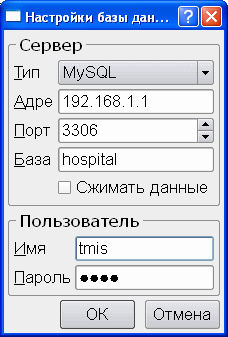
\includegraphics[width = 0.3\textwidth ,keepaspectratio]{cl_db}
 \caption{Настройка соединения с БД}
 \label{img_cl_db}
\end{figure} 

\begin{prim}
 По умолчанию все настройки клиентской части хранятся пользовательском каталоге. Для ОС Windows это папка <<C:$\backslash$Documents and Settings$\backslash$<имя пользователя>$\backslash$ Application Data$\backslash$ftmis-new$\backslash$>>, в файле <<ftmis-new.ini>>. Возможен перенос настроек клиентской части на другую машину простым копированием указанного файла в аналогичную папку на другом компьютере. Для создания нескольких вариантов пользовательских настроек ФТМИС на одной рабочей станции, необходимо в операционной системе создать несколько учетных записей пользователей. Для каждой учетной записи возможно сохранение собственных настроек клиентской части.
\end{prim}

\begin{vnim}
 В данном окне и при сохранении настроек соединения проверка доступности подключения не предусмотрена. Для проверки подключения следует в главном меню выбрать пункт \mm{Сессия \str Подключиться к базе данных}.
\end{vnim}

\subsection{Настройки умолчаний}

В разделе \dm{Умолчания} находятся все основные настройки, регулирующие работу пользователя в системе. Настройки данного раздела распространяются только на рабочую станцию (и пользователя), на которой они сохранены. Настройки хранятся в ini-файле профиля пользователя (например, в ОС Windows в папке <<C:$\backslash$Documents and Settings$\backslash$<имя поль\-зо\-ва\-те\-ля>$\backslash$Application Data$\backslash$ftmis-new$\backslash$ftmis-new.ini>>). Для настройки умолчаний нужно в главном меню выбрать пункт \mm{Настройки \str Умолчания}. Окно настройки состоит из нескольких вкладок (Рисунок \ref{img_cl_def}).

\begin{prim}
 В файле <<C:$\backslash$Documents and Settings$\backslash$<имя поль\-зо\-ва\-те\-ля>$\backslash$.ftmis-new$\backslash$error.log>> ведется протоколирование всех ошибок, возникающих на стороне клиента ФТМИС.
\end{prim}

\begin{figure}[ht]\centering
 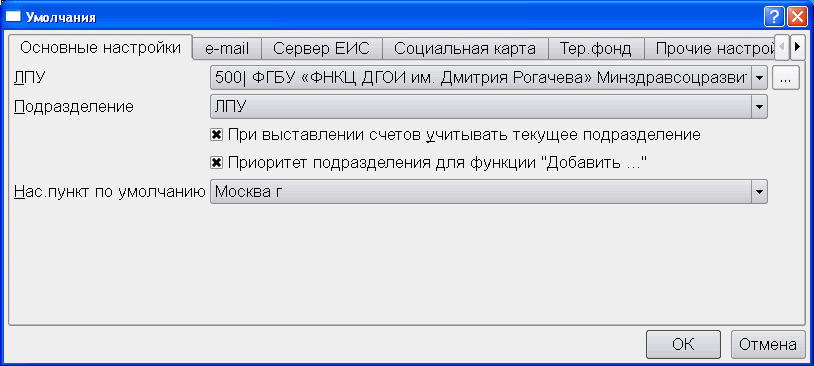
\includegraphics[width = 0.7\textwidth ,keepaspectratio]{cl_def}
 \caption{Настройка умолчаний}
 \label{img_cl_def}
\end{figure} 

На вкладке \dm{Основные настройки} указываются следующие параметры:
\begin{itemize}
 \item \dm{ЛПУ} – наименование базового ЛПУ, выбирается из справочника.
 \item \dm{Подразделение} – подразделение пользователя, выбирается из дерева ЛПУ. При выборе в данном поле значения <<ЛПУ>> для пользователей будет видна информация по всем подразделениям. При выборе определенного подразделения, пользователю будут видны только события и действия, разрешенные в выбранном и нижестоящих подразделениях.
 \item При установке флажка \dm{При выставлении счетов учитывать текущее подразделение} в окне формирования счетов в поле \dm{Подразделение} по умолчанию будет выставлено указанное выше подразделение, т.е. счета будут формироваться только по этому подразделению. При этом формирование счетов по другим подразделениям и ЛПУ в целом остается доступным.
 \item При установке флажка \dm{Приоритет подразделения для функции <<Добавить>>} по умолчанию будут автоматически подставляться действия, доступные для выбранного выше подразделения.
 \item \dm{Нас. пункт по умолчанию} – название населенного пункта следует выбрать из справочника КЛАДР. Данное название будет автоматически подставляться в поле адреса при регистрации новых пациентов, но его можно будет изменить. Данное значение так же будет использоваться для определения иногородних пациентов.
\end{itemize}

\begin{figure}[ht]\centering
 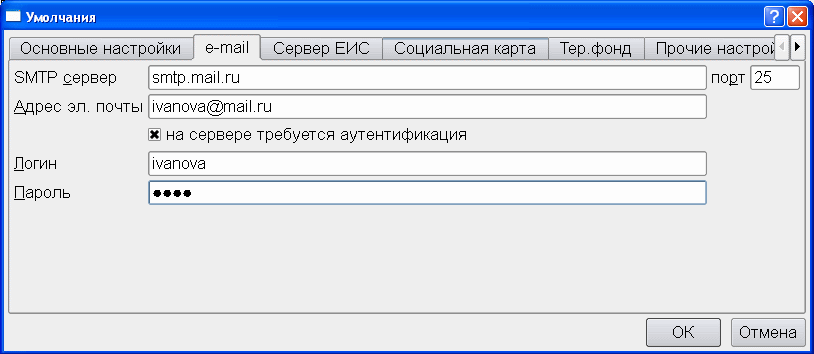
\includegraphics[width = 0.7\textwidth ,keepaspectratio]{cl_def_mail}
 \caption{Настройка почтового клиента}
 \label{img_cl_def_mail}
\end{figure} 

Вкладка \dm{e-mail} (Рисунок \ref{img_cl_def_mail}) содержит настройки встроенного почтового клиента ФТМИС. Он позволяет отправку отчетов и другой информации непосредственно из ФТМИС. Для корректной работы почтового клиента необходимо правильно заполнить следующие поля:
\begin{itemize}
 \item \dm{SMTP сервер};
 \item \dm{Порт};
 \item \dm{Адрес эл.почты} полностью;
 \item Флажок \dm{на сервере требуется аутентификация} позволяет ввести логин и пароль для доступа к учетной записи электронной почты;
 \item \dm{Логин} – имя пользователя электронной почты;
 \item \dm{Пароль} – пароль для доступа к электронной почте.
\end{itemize}

\begin{vnim}
 Отправка сообщений по почте возможна только если с текущей рабочей станции доступен SMTP-сервер эл. почты.
\end{vnim}
 
Вкладка \dm{Сервер ЕИС} содержит параметры соединения с сервером ЕИС региона (Рисунок \ref{img_cl_def_eis}). После заполнения всех необходимых полей соединения можно нажать кнопку \btn{Проверить соединение}, что позволит провести тест соединения.

\begin{figure}[ht]\centering
 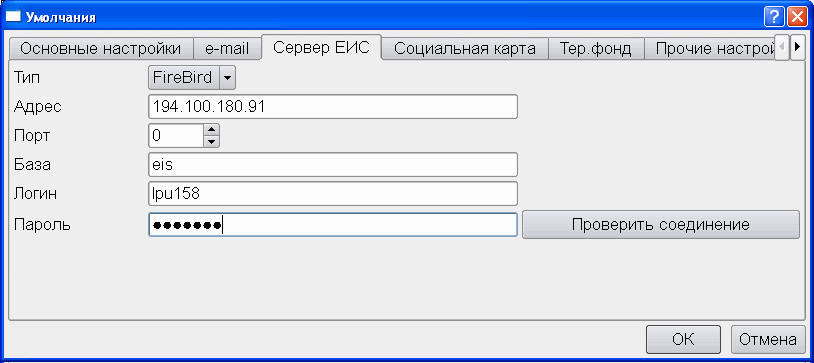
\includegraphics[width = 0.7\textwidth ,keepaspectratio]{cl_def_eis}
 \caption{Настройка соединения с ЕИС}
 \label{img_cl_def_eis}
\end{figure} 

Вкладка \dm{Социальная карта} содержит параметры подключения оборудования и справочников для работы с социальной картой пациента (Рисунок \ref{img_cl_def_sc}). Для того, чтобы поля данной вкладки стали доступны, необходимо установить флажок \dm{Включить поддержку социальной карты} в левом верхнем углу вкладки.

\begin{figure}[ht]\centering
 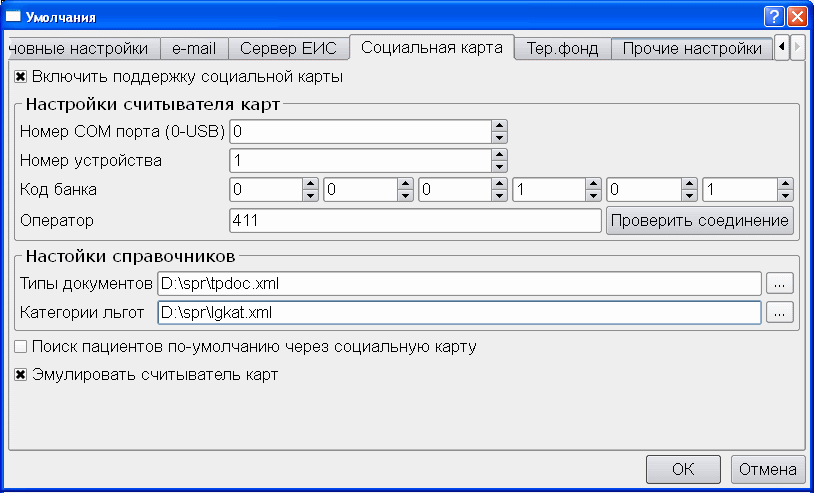
\includegraphics[width = 0.7\textwidth ,keepaspectratio]{cl_def_sc}
 \caption{Настройки работы с социальной картой}
 \label{img_cl_def_sc}
\end{figure} 

На вкладке \dm{Тер.фонд} содержатся настройки соединения с web-сервером ТФОМС региона для проверки действительности полиса пациента в базе застрахованных (Рисунок \ref{img_cl_def_tfoms}). Необходимо указать адрес сервера, а так же логин и пароль для доступа к данным. Для тестирования соединения можно воспользоваться кнопкой \btn{Проверить соединение}.

\begin{figure}[ht]\centering
 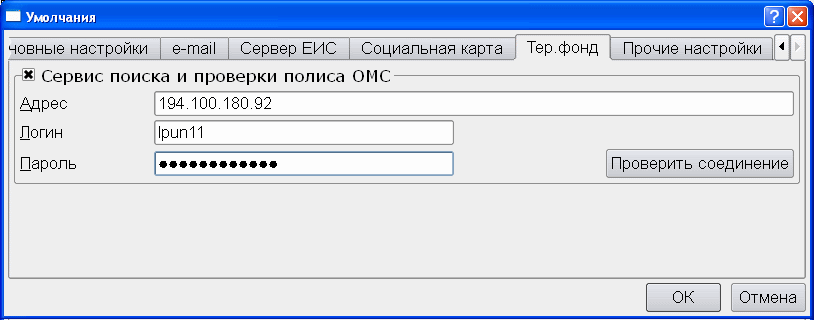
\includegraphics[width = 0.7\textwidth ,keepaspectratio]{cl_def_tfoms}
 \caption{Настройка соединения с сервером ТФОМС}
 \label{img_cl_def_tfoms}
\end{figure} 

Для того чтобы поля данной вкладки стали доступны для редактирования, нужно установить флажок \dm{Сервис поиска и проверки полиса ОМС} в левом верхнем углу вкладки. После установки и сохранения данного флажка в регистрационной карточке пациента, в разделе \dm{Полис ОМС} станет доступной кнопка \btn{Искать}, при нажатии на которую осуществляется поиск полиса в базе данных ТФОМС (Рисунок \ref{img_cl_card_tfoms}).

\begin{figure}[ht]\centering
 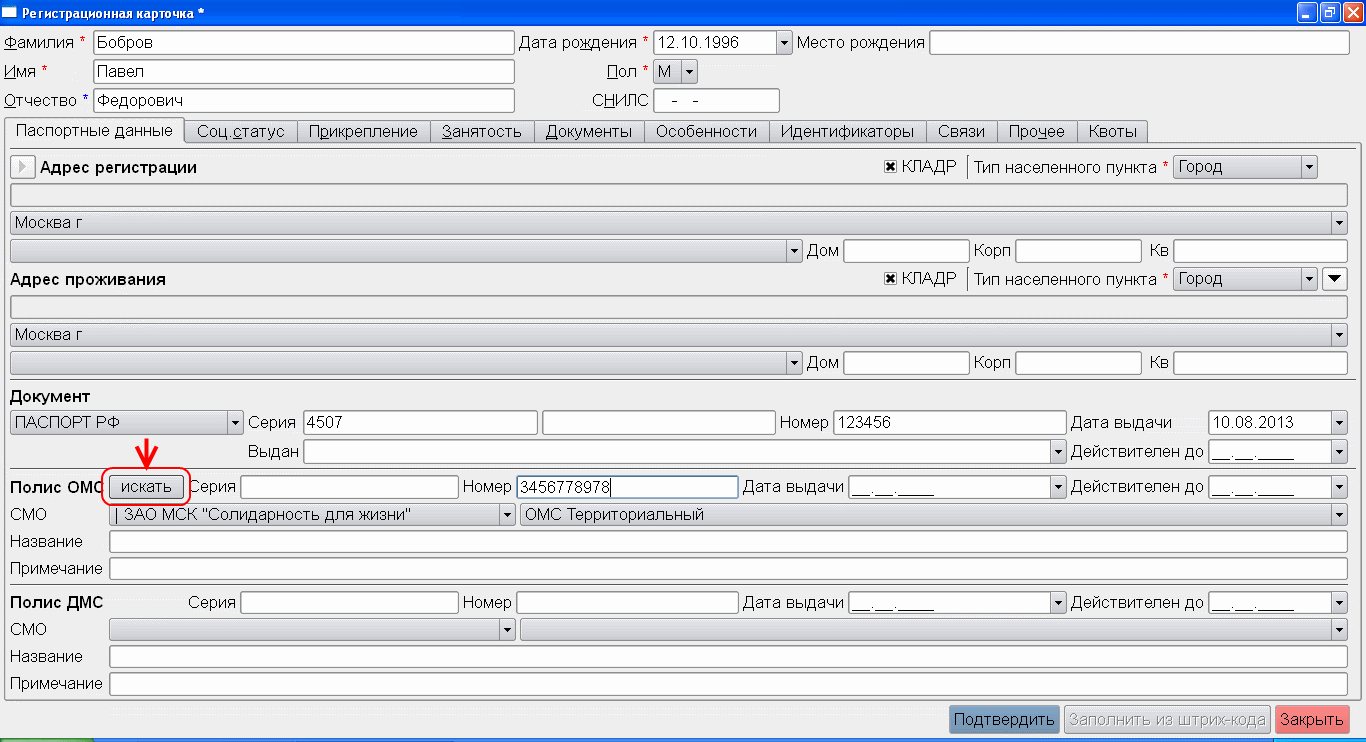
\includegraphics[width = 1\textwidth ,keepaspectratio]{cl_card_tfoms}
 \caption{Кнопка проверки страхового полиса в регистрационной карточке пациента}
 \label{img_cl_card_tfoms}
\end{figure} 

На вкладке \dm{Прочие настройки} содержатся специальные настройки реакции на различные события клиентского приложения (Рисунок \ref{img_cl_def_oth}). Описание опций настройки приведено в таблице \ref{tbl_def1}.

\begin{figure}[ht!]\centering
 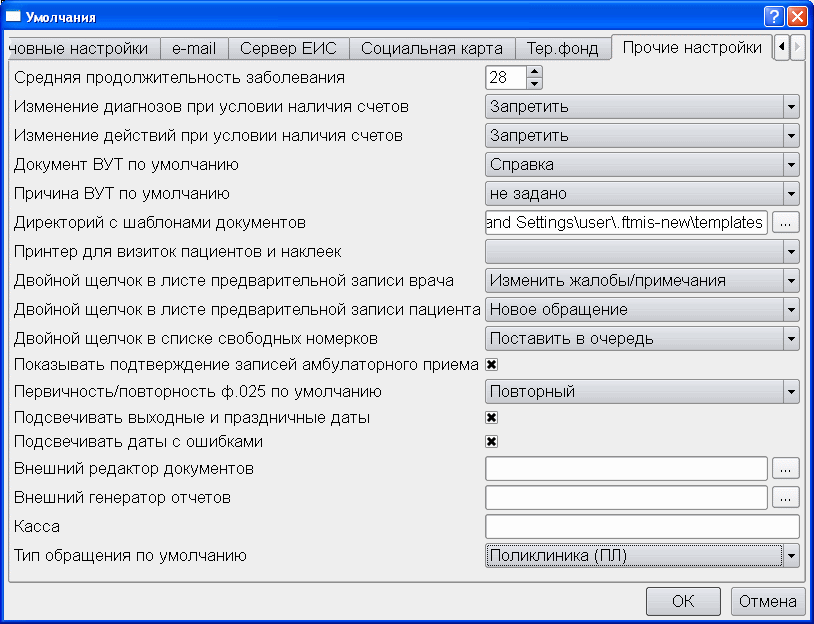
\includegraphics[width = 0.7\textwidth ,keepaspectratio]{cl_def_oth}
 \caption{Вкладка <<Прочие настройки>>}
 \label{img_cl_def_oth}
\end{figure} 

{\small
\begin{longtable}{|p{5cm}|p{11.8cm}|}
\caption{Настройка умолчаний. Вкладка <<Прочие настройки>> \label{tbl_def1}}\\
\hline \rule{0pt}{15pt} \hfil \textbf{Опция} & \hfil \textbf{Описание}\\ \hline
\endfirsthead
\hline \rule{0pt}{15pt} \hfil \textbf{Опция} & \hfil \textbf{Описание}\\ \hline
\endhead
Средняя продолжительность заболевания & Средняя продолжительность заболеваний для отчетов \\ \hline
Изменение диагнозов при условии наличия счетов & Разрешает или запрещает изменение диагнозов в обращениях, по которым уже выставлен счет \\ \hline
Изменение действий при условии наличия счетов &	Разрешает или запрещает изменение состава обращения после выставления счета \\ \hline
Документ ВУТ по умолчанию &	Значение, подставляемое по умолчанию при создании документа ВУТ \\ \hline
Причина ВУТ по умолчанию &	Значение, подставляемое по умолчанию при создании документа ВУТ \\ \hline
Директорий с шаблонами документов &	В поле указывается путь к папке с шаблонами печатных форм (в случае их размещения локально). Можно использовать кнопку \btn{\rule{0pt}{5pt}…} для указания пути \\ \hline
Принтер для визиток пациентов и наклеек	& Выбирается из списка принтеров, установленных на данной рабочей станции \\ \hline
Двойной щелчок в лис\-те предварительной записи врача &	Реакция на двойной щелчок мыши на панели \dm{График} по фамилии пациента, записанного на прием (Рисунок \ref{img_cl_def_work}, позиция 1) \\ \hline
Двойной щелчок в лис\-те предварительной записи пациента &	Реакция на двойной щелчок мыши по записи на вкладке \dm{Пациенты} в разделе \dm{Предварительная запись} окна обслуживания пациентов (Рисунок \ref{img_cl_def_work}, позиция 2) \\ \hline
Двойной щелчок в списке свободных номерков	& Реакция на двойной щелчок по свободному номерку на панели \dm{График} или \dm{Номерки} (при условии, что в картотеке пациентов выбран пациент) (Рисунок \ref{img_cl_def_work}, позиция 3) \\ \hline
Показывать подтверждение записей амбулаторного приема	& При установке данного флажка на панели \dm{График} в списке пациентов, записанных на прием, слева от фамилии пациентов появляется дополнительный флажок подтверждения (Рисунок \ref{img_cl_work_acc}) \\ \hline
Первичность/повторность ф.025 по умолчанию	& При создании нового обращения в поле \dm{Первичность} по умол\-ча\-нию указывается выбранное значение \\ \hline
Подсвечивать выходные и праздничные даты	& Во всех полях для указания дат регистрационной карточки пациента, карточки обращения и др. выходные и праздничные дни окрашиваются в красный цвет (Рисунок \ref{img_cl_work_dat}) \\ \hline
Подсвечивать даты с ошиб\-ка\-ми	& Во всех полях для указания дат регистрационной карточки пациента, карточки обращения и др. неправильные (несуществующие) даты окрашиваются в малиновый цвет (Рисунок \ref{img_cl_work_dat}) \\ \hline
Внешний редактор документов	& Путь к исполняемому файлу приложения для редактирования документов (используется для редактирования печатных форм, вызывается из окна предварительного просмотра печатной формы) \\ \hline
Внешний генератор отчетов	& Путь к исполняемому файлу приложения генерации отчетов. Данный редактор вызывается из главного меню \mm{Анализ \str Генератор отчетов} \\ \hline
Касса &	Если рабочая станция расположена в кассе, то в данном поле необходимо ввести с клавиатуры название кассы. Указанное название будет использоваться в качестве названия кассы во всех кассовых операциях \\ \hline
Тип обращения по умолчанию	& При создании нового обращения в поле \dm{Тип обращения} по умолчанию подставляется выбранное значение. Значение выбирается из списка. Состав списка определяется настройкой справочника \dm{Типы обращений} \\ \hline
\end{longtable}
}

\begin{figure}[ht!]\centering
 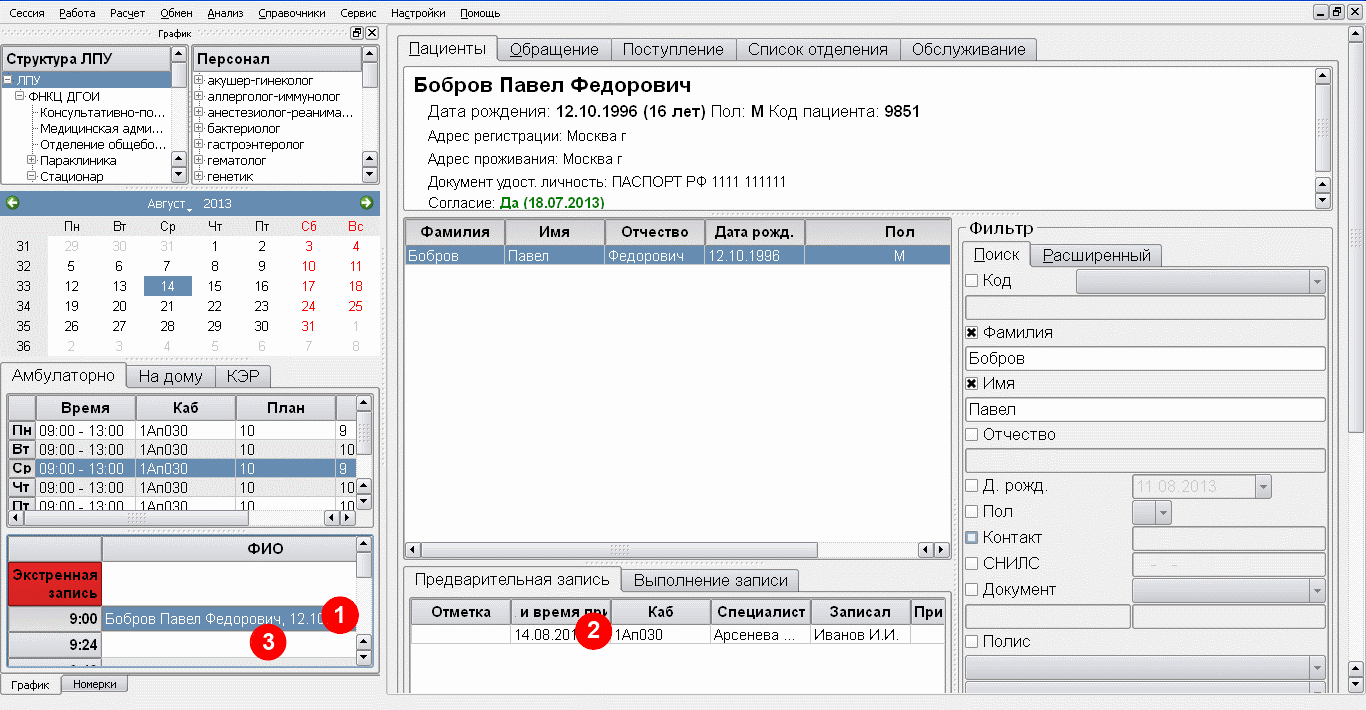
\includegraphics[width = 1\textwidth ,keepaspectratio]{cl_def_work}
 \caption{Позиции, реакция на которые предусмотрена в настройках}
 \label{img_cl_def_work}
\end{figure}

\begin{figure}[ht!]\centering
 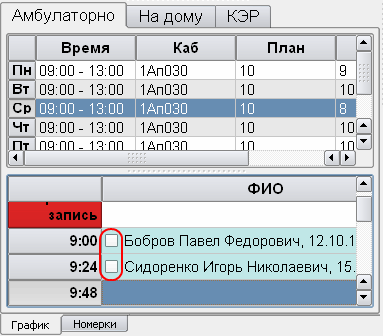
\includegraphics[width = 0.5\textwidth ,keepaspectratio]{cl_work_acc}
 \caption{Подтверждение записей амбулаторного приема}
 \label{img_cl_work_acc}
\end{figure}

\begin{figure}[ht!]\centering
 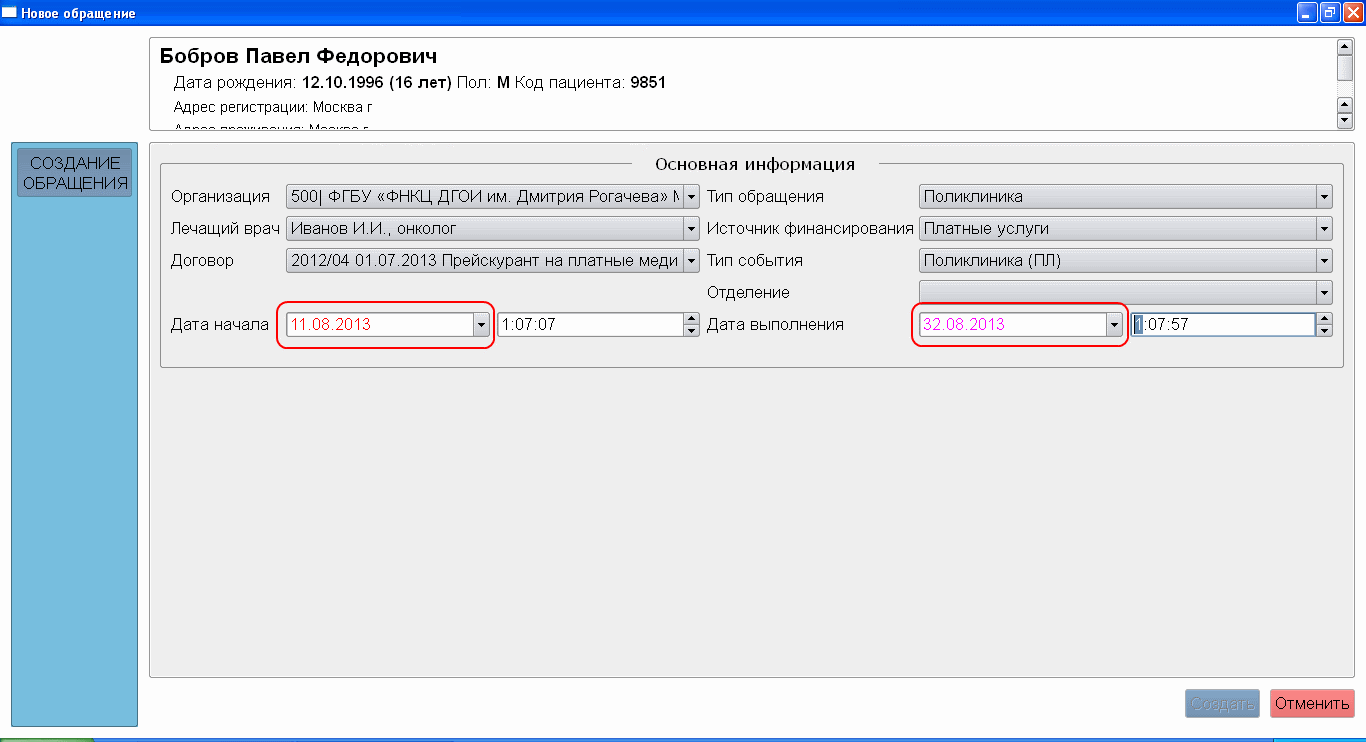
\includegraphics[width = 1\textwidth ,keepaspectratio]{cl_work_dat}
 \caption{Подсвечивание дат}
 \label{img_cl_work_dat}
\end{figure}

\subsection{Настройка внешнего вида}

Настройки внешнего вида приложения так же производится отдельно для каждой рабочей станции. Для открытия окна настройки необходимо в главном меню выбрать пункт \mm{Настройки \str Внешний вид} (Рисунок \ref{img_cl_vid}).

\begin{figure}[ht!]\centering
 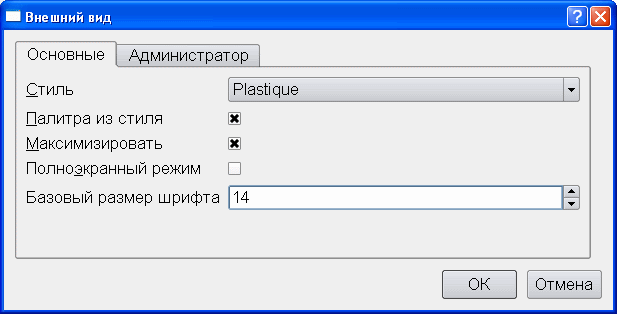
\includegraphics[width = 0.6\textwidth ,keepaspectratio]{cl_vid}
 \caption{Настройка внешнего вида приложения}
 \label{img_cl_vid}
\end{figure}

В открывшемся окне можно указать следующие параметры:
\begin{itemize}
 \item \dm{Стиль} оформления окон приложения выбирается из фиксированного списка стилей.
 \item Флажок \dm{Палитра стиля} позволяет использовать цвета оформления окон, заданные в выбранном стиле.
 \item Флажок \dm{Максимизировать} обеспечивает раскрытие на весь экран окна приложения при запуске.
 \item Флажок \dm{Полноэкранный режим} позволяет запустить приложение во весь экран. Панель задач при этом будет недоступной, а окно приложения невозможно будет свернуть.
 \item \dm{Базовый размер шрифта} – размер шрифта основного текста на экране.
\end{itemize}
 
После внесения изменений, настройки необходимо сохранить, нажав кнопку \btn{OK}. %Настройки клиентской части
  \newpage
\section{Подсистема справочников}

Подсистема справочников предоставляет инструменты для ведения единых справочников, которые совместно используются  \tmis и интегрируемыми подсистемами.

При переходе в подсистему справочников открывается главная страница подсистемы (Рисунок \ref{img_spr_main}).

\begin{figure}[ht]\centering
 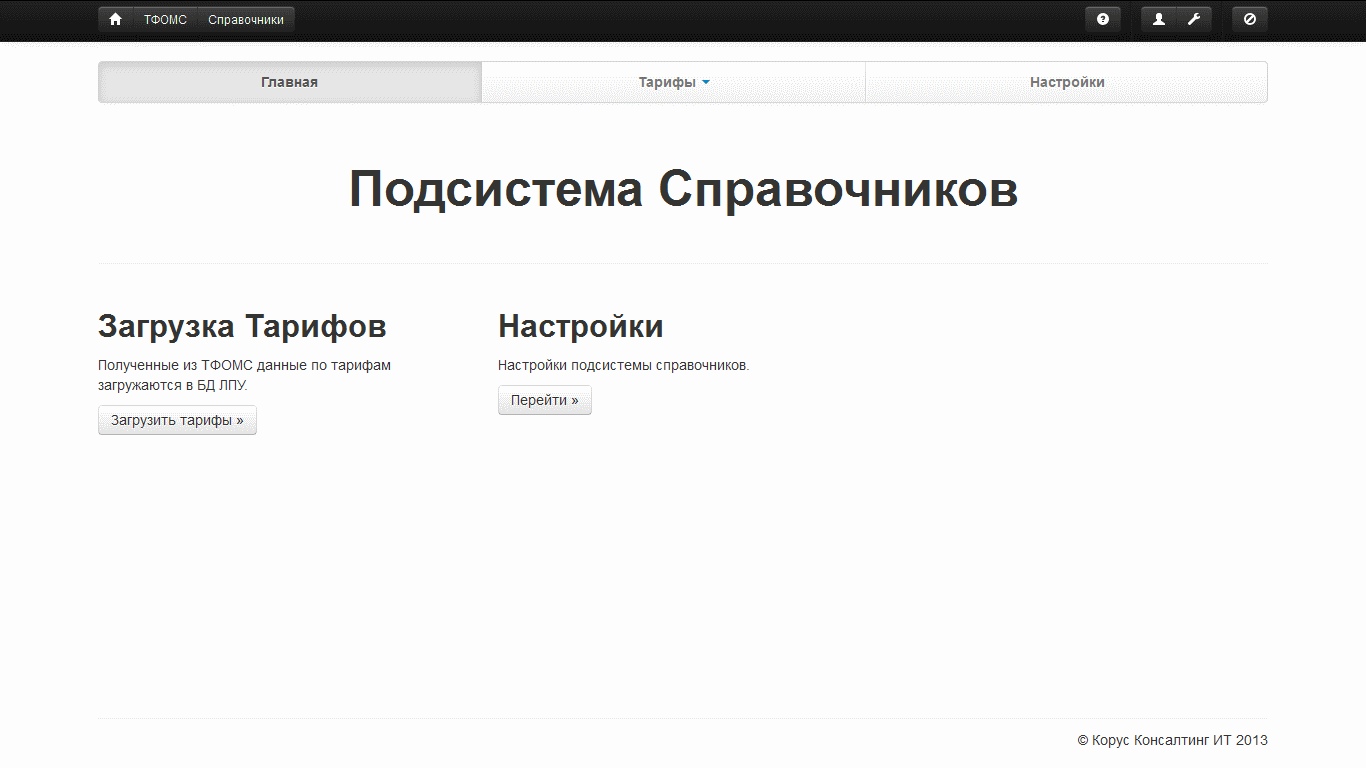
\includegraphics[width = 1\textwidth ,keepaspectratio]{spr_main}
 \caption{Главная страница подсистемы справочников}
 \label{img_spr_main}
\end{figure}

\subsection{Настройки подсистемы}

Для перехода на страницу настройки подсистемы ведения справочников нужно нажать кнопку \btn{Настройки}  в верхней части любой страницы, либо нажать кнопку  \btn{Перейти >>} в разделе \dm{Настройки} на главной странице подсистемы.

Страница настроек подсистемы имеет следующий вид (Рисунок \ref{img_spr_conf}).

\begin{figure}[ht]\centering
 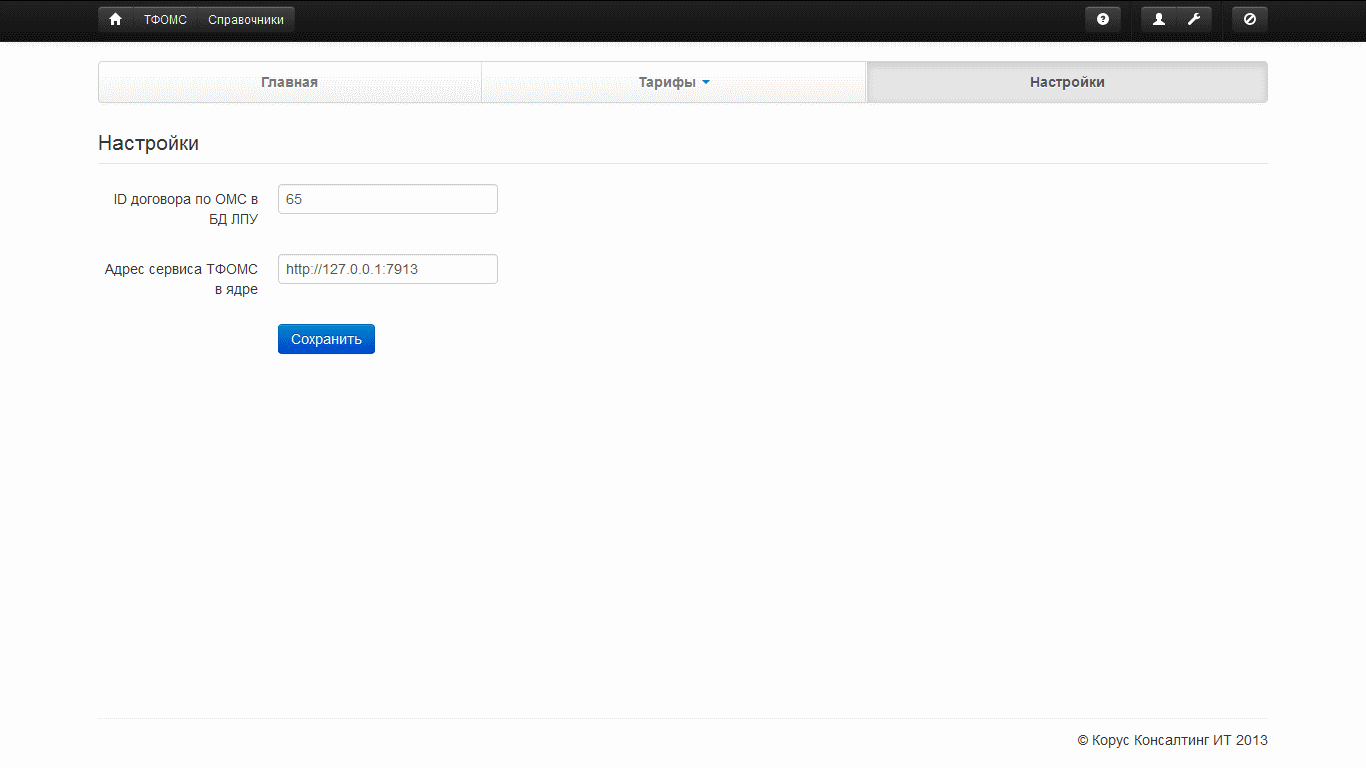
\includegraphics[width = 1\textwidth ,keepaspectratio]{spr_conf}
 \caption{Настройки подсистемы справочников}
 \label{img_spr_conf}
\end{figure}
 
 %Настройка справочников
  \newpage
\normalsize
\section{Создание шаблонов печатных форм}

\tmis~предоставляет широкие возможности по созданию и форматированию пользовательских печатных форм. Благодаря наличию в системе шаблонизаторов, администратор системы может создавать печатные формы любых медицинских документов в соответствии с требованиями пользователей.

Для создания шаблонов печатных форм необходимо:
\begin{enumerate}
 \item Владеть основами языка HTML.
 \item Знать синтаксис выбранного шаблонизатора.
 \item Иметь список объектов соответствующего контекста печати.
\end{enumerate}
 
Язык HTML используется для форматирования шаблона печатной формы. Получение данных из БД осуществляется через объекты контекста печати. Синтаксис языка позволяет создавать циклические структуры, вывод значений объектов по условию, представление объектов в определенном формате.

\subsection{Регистрация шаблонов печатных форм в \tmis} \label{patt_add}

Шаблоны печатных форм могут храниться в БД либо на рабочей станции (в папке указанной в поле \dm{Директорий с шаблонами документов} на вкладке \dm{Прочие} настройки окна настройки умолчаний, вызываемого из  меню \mm{Настройки \str Умолчания}). При наличии одновременно одноименного шаблона печатной формы в БД и на рабочей станции, будет использоваться шаблон с рабочей станции.

Управление шаблонами печатных форм осуществляется из главного меню в пункте \mm{Настройки \str Шаблоны печати}. Открывающееся окно представляет собой  справочник шаблонов печатных форм, использующихся в системе (Рисунок \ref{img_patt_list}). В нем перечислены как шаблоны, сохраненные в БД, так и шаблоны, хранящиеся на рабочих станциях. Здесь же осуществляется связь шаблона печатной формы с местом его вызова в приложении.

\begin{figure}[ht]\centering
 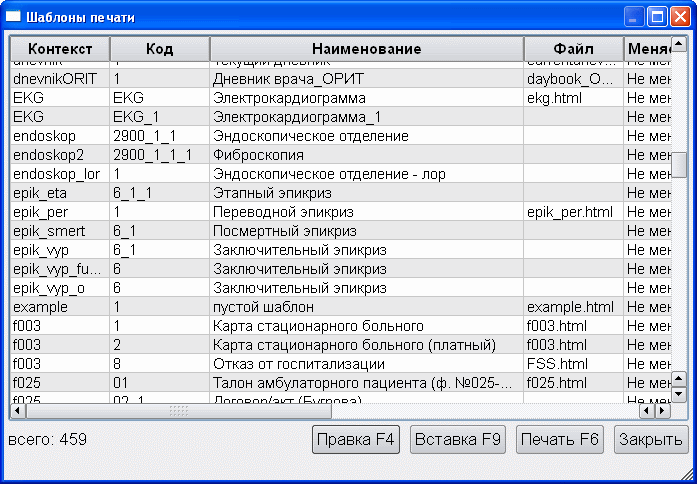
\includegraphics[width = 0.7\textwidth ,keepaspectratio]{patt_list}
 \caption{Список шаблонов печатных форм}
 \label{img_patt_list}
\end{figure}

\begin{figure}[ht]\centering
 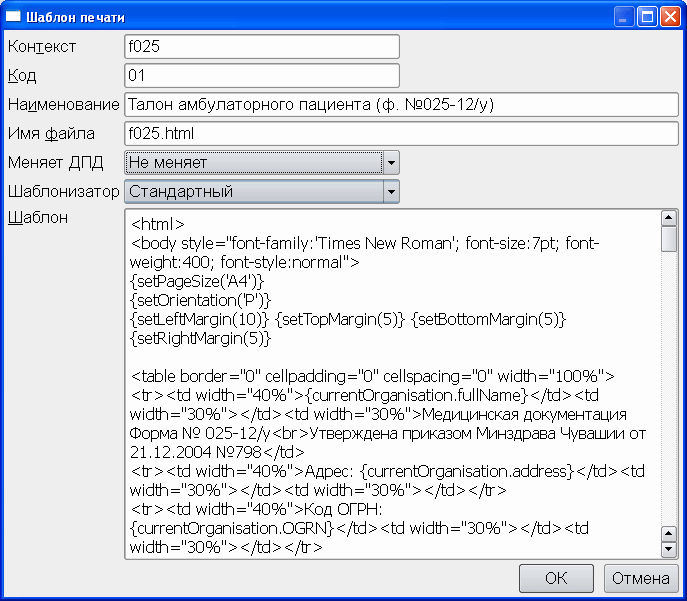
\includegraphics[width = 0.7\textwidth ,keepaspectratio]{patt_card}
 \caption{Карточка редактирования шаблона печати}
 \label{img_patt_card}
\end{figure}

Для регистрации нового шаблона печатной формы нужно нажать кнопку \btn{Вставка F9}. В открывшемся окне (Рисунок \ref{img_patt_card}) следует указать следующие параметры:
\begin{itemize}
 \item \dm{Контекст} – наименование контекста печати. С помощью данного поля происходит определение места вызова печатной формы. Как правило, печатные формы вызываются из карточки редактирования события (вкладка \dm{Основная информация}) или действия при нажатии кнопки \btn{Печать}. Для того чтобы шаблон печати вызывался из карточки редактирования определенного типа события (или действия) необходимо, чтобы значение данного поля совпадало со значением поля \dm{Контекст печати} справочника \dm{Типы событий} (\dm{Типы действий}). Рекомендуется в качестве значений поля \dm{Контекст} использовать короткие сочетания цифр, английских букв, знаков тире и подчеркивание. Существуют так же предопределенные значения контекста. Например, при указании значения <<token>>, шаблон печати будет вызываться из окна картотеки пациентов.
 \item \dm{Код} – для каждого контекста печати может быть задано несколько шаблонов печатных форм. Значение данного поля задает последовательность расположения шаблонов печати в контекстном меню кнопки \btn{Печатать} заданного окна.
 \item \dm{Наименование} – название печатной формы, отображаемое в контекстном меню кнопки \btn{Печатать}.
 \item \dm{Имя файла} – название файла шаблона печатной формы, если он хранится на рабочей станции.
 \item \dm{Меняет ДПД} – задает изменение значения идентификатора ДПД при вызове печати данного шаблона. Так, для печатных форм типа <<Информированное согласие …>> рекомендуется устанавливать значение данного поля в <<Меняет на <<Да>>. Тогда после печати формы на основе данного шаблона, в карточке пациента будет сделана отметка о получении от него согласия на проведение лечения.
 \item \dm{Шаблонизатор} – выбор типа шаблонизатора из списка. В зависимости от выбранного типа, нужно использовать различный синтаксис при создании шаблона печатной формы.
 \item \dm{Шаблон} – скрипт шаблона печатной формы, сохраняемый в БД.
\end{itemize}

\subsection{Структура шаблонов печатных форм}

Любой шаблон печатной формы представляет собой html-скрипт, содержащий специальные переменные и выражения. Переменные и выражения оформляются в соответствии с синтаксисом выбранного типа шаблонизатора.

На текущий момент \tmis~поддерживается 2 типа шаблонизаторов, синтаксис которых различен:
\begin{enumerate}
 \item Стандартный;
 \item Jinja2.
\end{enumerate}
 
При настройке новых шаблонов печатных форм рекомендуется использовать шаблонизатор jinja2, т.к. он предоставляет более широкие возможности по созданию шаблонов.

\subsubsection{Синтаксис стандартного шаблонизатора}

При использовании стандартного шаблонизатора все операторы и выражения обрамляются в фигурные скобки. Например, \code{\{setPageSize ('A4')\}} или \code{\{for: prop in action\}}.

В общем случае, операторы могут иметь следующий формат:
\code{\{<ключевое слово>:<выражение>\}} или \code{\{<выражение>\}}.

В качестве ключевых слов могут быть использованы: \code{if}, \code{elif}, \code{else}, \code{for}, \code{end}.

При использовании первого варианта выражения (с ключевым словом), значение выражения определяется ключевым словом.

При использовании второго варианта выражения (без ключевого слова), оно, как правило, выполняет роль оператора вывода на печать. Например, \code{\{client.fullName\}} – вывод на печать ФИО пациента. Исключением является установка опций печати, например, \code{\{setPageSize('A4')\}}.

Если в выражении используются строки, то необходимо использовать префикс <<u>> (unicode), например \code{\{if: action.name == u"Поступление"\}\{: currentAction = action\}\{end:\}}.

Конструкция \verb|{#<комментарий>#}| позволяет закомментировать часть текста.

Опции, задающие формат листа для печати:
\begin{itemize}
 \item \verb|{setPageSize('A4')}| – размер листа для печати;
 \item \verb|{setOrientation('P')}| – ориентация листа при печати: <<P>> – книжная, <<L>> – альбомная;
 \item \verb|{setMargins(10)}| – задает поля листа (одинаковое поле со всех сторон);
 \item \verb|{setLeftMargin(15)}| – задает левое поле;
 \item \verb|{setRightMargin(15)}| – задает правое поле;
 \item \verb|{setTopMargin(15)}| – задает верхнее поле;
 \item \verb|{setBottomMargin(15)}| – задает нижнее поле.
\end{itemize}

\paragraph{Оператор условия}

Общий вид оператора условия: 
\begin{verbatim}
{if: <условие>} 
<действие1> [<действие2>] … [<действиеN]
<!--Выполняются при выполнении условия --> 
[{elif: <условие2 (проверяется, если не выполнилось основное условие>} 
<действие2_1> [<действие2_2>] … [<действие2_N]] 		
<!-- Выполняются, если основное условие не выполняется, а условие2
 выполняется  --> 
[{else:} 
<действие3_1> [<действие3_2>] … [<действие3_N]] 	
<!—Выполняются, если основное условие и условие2 не выполнены --> 
{end:} 
\end{verbatim}

При задании условия могут использоваться операторы сравнения: == (равно), != (не равно), <, >, <=, >=. Могут быть использованы сложные условия, объединенные с помощью ключевых слов \code{AND}, \code{OR}, \code{NOT}. \\

\opr{Пример1:} ~Для первой позиции в списке печатается значение <<Первая позиция>>, для остальных – <<Последующая позиция>>.
\begin{verbatim}
{if: k==0}{:k=1} 
<hr>Первая позиция <br>
{else:}
{:k=k+1}
Последующая позиция <br>
{end:}
\end{verbatim}

\opr{Пример2:} ~Если наименование текущего действия<<Поступление>>, то ссылка на него сохраняется в переменной \code{currentAction}.
\begin{verbatim}
{if: action.name == u"Поступление"}{: currentAction = action}{end:}
\end{verbatim}

Существует еще один вариант организации условия в стандартном шаблонизаторе. Принцип его работы аналогичен функции \code{iif} во многих языках программирования. В общем виде он выглядит следующим образом:

\verb|{<действие1> if <условие> else <действие2>}|

Описанная функция может использоваться как в качестве действия, так и в качестве части действия. Например: \begin{verbatim}
{: string = u"д. " + client.regAddress.number +
 ((u" корп. " + client.regAddress.corpus) 
 if (client.regAddress.corpus != "") else "") + u" кв. " +
  client.regAddress.flat}.
\end{verbatim} 
В описанном примере функция условия (помещена в круглые скобки) добавляет в адресную строку информацию о корпусе, только если это поле заполнено.

\paragraph{Оператор цикла} 

Общий вид оператора цикла:
\begin{verbatim}
{for: <переменная цикла> in <область значений переменной>}
<действие1>
[<действие2>]
…
[<действиеN>]
{end:}
\end{verbatim}

\opr{Пример3}: ~Поиск действия <<Поступление>> среди действий события.
\begin{verbatim}
{for: action in event.actions}
{if: action.name == u"Поступление"}{: currentAction = action}{end:}
{end:}
\end{verbatim}

\subsubsection{Организация диалогов}

При создании отчетов можно организовать получение входных значений посредством организации диалогов с пользователем. Для отображения диалогового окна следует использовать объект \code{dialogs}. В зависимости от выбранного метода, в результате работы диалога будет получено значение переменной определенного типа. Например, \code{\{: StrKod = dialogs.dialString(u"Введите код МКБ заболевания").getVar()\}} позволяет получить значение кода МКБ заболевания в виде строки. Можно использовать следующие методы объекта \code{dialogs}:
\begin{itemize}
 \item \code{dialBool} – диалог ввода логического значения;
 \item \code{dialDate} – диалог ввода даты;
 \item \code{dialFloat} – диалог ввода числа с плавающей точкой;
 \item \code{dialInt} – диалог ввода целого числа;
 \item \code{dialList} – диалог выбора значения из списка;
 \item \code{dialMultiList} – диалог выбора множественных значений из списка;
 \item \code{dialString} – диалог ввода строки;
 \item \code{dialTime} – диалог ввода времени.
\end{itemize}
 
Для всех перечисленных типов диалогов в качестве первого параметра указывается название диалога. Для методов \code{dialList} и \code{dialMultiList} указывается так же второй параметр – список значений в квадратных скобках. Для получения выбранного значения следует использовать метод \code{getVar()}.

\subsubsection{Функции работы с датами}

Функции определения текущей даты и времени:
\begin{itemize}
 \item \verb|{currentDate}| – текущая дата;
 \item \verb|{currentTime}| – текущее время.
\end{itemize}
 
Для задания формата вывода даты и времени используются методы \\ \code{date.toString(<формат>)} и \code{time.toString(<формат>)}. Например, \\ \code{action.endDate.date.toString('dd.MM.yyyy')} или  \code{action.begDate.time. toString('hh:mm')}.

Метод \code{daysTo(<конечная дата>)} возвращает количество дней от указанной даты до конечной. Например, \code{event.setDate.date.daysTo(currentDate. date)}.

Метод \code{addDays(<количество>)} увеличивает (либо уменьшает при указании отрицательного числа) дату на указанное количество дней. Например, \code{\{: currDate = act.begDate.date.addDays(1)\}} показывает день, следующий за \code{begDate}.

\subsection{Синтаксис шаблонизатора Jinja2}

В качестве альтернативы стандартному шаблонизатору в \tmis~был добавлен шаблонизатор jinja2. В отличии от стандартного шаблонизатора, который является частью \tmis, jinja2 разрабатывается и поддерживается командой сторонних разработчиков. Это достаточно крупный проект с открытым исходным кодом (open source). Jinja2 предоставляет более широкие возможности для разработки шаблонов. Конструкции языка соответствуют общепринятым стандартам, более четкие и выверенные по сравнению со стандартным шаблонизатором.

Синтаксис шаблонизатора jinja2 имеет общие черты с синтаксисом стандартного шаблонизатора, но имеет и заметные отличия.

В шаблонизаторе jinja2 операторы могут обрамляться в двойные фигурные скобки \verb|{{ … }}| или фигурные скобки и знаки процента \verb||. Например, \code{\{\{setPageSize('A4')\}\}} или \code{\{\%for: prop in action\%\}}. Обрамление \verb|| используется для исполняемых операторов. Обрамление \verb|{{ … }}|, выполняет роль оператора вывода на печать. В обрамлении \verb|{# … #}| записываются комментарии.

\begin{vnim}
 В отличии от стандартного шаблонизатора, в Jinja2 не нужно добавлять префикс <<u>> перед строками. Например,  \{\%if action.name == "Поступление"\%\} \{\% currentaction = action \%\} \{\% endif \%\}
\end{vnim}
 
В jinja2 существует 2 способа обращения к свойствам переменных:
\begin{enumerate}
 \item \verb|{{new_var.prop1}}|;
 \item \verb|{{new_var['prop1']}}|.
\end{enumerate}

Оба они позволяют получить значение свойства переменной, однако, во втором случае сначала будет осуществляться поиск записи \verb|'prop1'| в \verb|new_var|, а только затем поиск свойства \verb|prop1|. В первом случае поиск происходит в обратном порядке.

Опции, задающие формат листа для печати:
\begin{itemize}
 \item \verb|{{setPageSize('A4')}}| – размер листа для печати;
 \item \verb|{{setOrientation('P')}}| – ориентация листа при печати: «P» – книжная, «L» – альбомная;
 \item \verb|{{setMargins(10)}}| – задает поля листа (одинаковое поле со всех сторон);
 \item \verb|{{setLeftMargin(15)}}| – задает левое поле;
 \item \verb|{{setRightMargin(15)}}| – задает правое поле;
 \item \verb|{{setTopMargin(15)}}| – задает верхнее поле;
 \item \verb|{{setBottomMargin(15)}}| – задает нижнее поле.
\end{itemize}
 
\subsubsection{Оператор условия}

Общий вид оператора условия:
\begin{verbatim}

<действие1> [<действие2>] … [<действиеN]	{# Выполняются при 
выполнении условия #}
[
<действие2_1> [<действие2_2>] … [<действие2_N]]	{# Выполняются, если
 основное условие не выполняется, а условие2 выполняется #}
[
<действие3_1> [<действие3_2>] … [<действие3_N]]	{# Выполняются, если
 основное условие и условие2 не выполнены #}

\end{verbatim}

Следует обратить внимание, что в Jinja условный оператор всегда заканчивается ключевым словом \code{endif}, а не \code{end}, как в стандартном шаблонизаторе.

При задании условия могут использоваться операторы сравнения: == (равно), != (не равно), <, >, <=, >=. Могут быть использованы сложные условия, объединенные с помощью ключевых слов \code{AND}, \code{OR}, \code{NOT}.

\opr{Пример4:} ~Выводится значение k. Если оно отрицательное, то печатается жирным (без знака). Если оно равно нулю, то значение выводится текстом.
\begin{verbatim}

<li>{{k}}</li>

<li><b>{{-k}}</b></li>

<li>Ноль</li>

\end{verbatim}

\subsubsection{Оператор цикла}

Общий вид оператора цикла:
\begin{verbatim}

<действие1>
[<действие2>]
…
[<действиеN>]

\end{verbatim}

Как и в предыдущем пункте, цикл заканчивается специальным ключевым словом \code{endfor}.

\opr{Пример5:} ~Вывод на печать значений свойств.
\begin{verbatim}
 
<td align="left">{{prop[0]}}</td> 
<td align="center">{{prop[2]}}</td>

\end{verbatim}

\subsubsection{Организация диалогов}

При создании отчетов с параметрами можно организовать диалоги с пользователем. Для отображения диалогового окна следует использовать объект \code{dialogs}. В зависимости от выбранного метода, в результате работы диалога будет получено значение переменной определенного типа. Например, \verb|| позволяет получить значение переменной \code{DataVVn} типа дата. Список методов объекта \code{dialogs} приведен в таблице \ref{tbl_patt_jdlg}.

{\small
\begin{longtable}{|p{3cm}|p{4.7cm}|p{9cm}|}
\caption{Типы диалогов \label{tbl_patt_jdlg}} \\
\hline \rule{0pt}{15pt} \centering \textbf{Название} & \centering \textbf{Аргументы} & \hfil \textbf{Описание} \\ \hline
\endfirsthead
\hline \rule{0pt}{15pt} \centering \textbf{Название} & \centering \textbf{Аргументы} & \hfil \textbf{Описание} \\ \hline
\endhead
dialBool &	Название диалога	& Ввод значения переменной логического типа  \\ \hline
dialDate &	Название диалога &	Ввод значения переменной типа дата \\ \hline
dialInt	& Название диалога	& Ввод значения целочисленной переменной \\ \hline
dialFloat &	Название диалога &	Ввод значения переменной с плавающей точкой \\ \hline
dialMultiList &	Название диалога, список значений &	Выбор нескольких значений из списка. Список доступных значений заключается в квадратные скобки. Для получения значения функции, следует применять метод \code{getListValues()}. Например, \code{dialogs.dialMultiList("Выберите элемент (ы) из списка}\verb|",["1", "2", "3"]).| \code{getListValues()} \\ \hline
dialList	& Название диалога, список значений	& В отличии от предыдущего элемента, в данном случае можно выбрать только одно значение из предложенного списка \\ \hline
dialOrg	& Название диалога	& Выбор значения переменной из справочника организаций \\ \hline
dialOrgStructure	& Название диалога	& Выбор подразделения из организационной структуры ЛПУ \\ \hline
dialPerson	& Название диалога &	Выбор сотрудника из справочника сотрудников \\ \hline
dialRB	& Название диалога, название таблицы БД справочника	& Выбор значения переменной из справочника, название которого указано в качестве второго аргумента (название справочника указывается в двойных кавычках). В данном типе диалога могут быть использованы следующие методы: \begin{itemize}
 \item \code{getId()} – возвращает идентификатор выбранной записи;
 \item \code{getCode()} – возвращает код выбранной записи (из поля Code справочника);
 \item \code{getName()} – возвращает название элемент справочника;
 \item \code{getVar()} – возвращает значение элемента справочника (поле \code{Code} либо его аналог), может использоваться для справочников, не имеющих поля \code{Code}.
\end{itemize}  
Например, \code{dialogs.dialRB("Выберите вид полиса"}\verb|, "rbPolicyType").getCode()| \\ \hline
dialService	& Название диалога	& Выбор услуги из справочника \mm{Услуга (профиль ЕИС)}. Могут быть использованы методы \code{getId()}, \code{getCode()}, \code{getName()}, описанные в предыдущем пункте \\ \hline
dialString	& Название диалога	& Ввод значения переменной символьного типа (строки) \\ \hline
dialTime	& Название диалога &	Ввод значения переменной типа время \\ \hline
\end{longtable}
}

Для получения значения в типах диалогов, для которых в таблице \ref{tbl_patt_jdlg} не указаны доступные методы, следует использовать метод \code{getVar()}.

\subsubsection{Использование фильтров}

Фильтрами в jinja называются функции преобразования (изменения) переменных. Например, преобразования типов, обработки строк, форматирования, математические функции и др.

В общем виде применение фильтра выглядит следующим образом:
\begin{verbatim}
<результирующая переменная> = <исходная
переменная>|функция[(<аргумент2>[,<аргумент3>…[,<аргументN>]])]
\end{verbatim}

Т.е. в начале указывается переменная, к которой следует применить фильтр (функцию), затем ставится вертикальная черта и указывается название фильтра. В скобках после названия фильтра могут указываться дополнительные аргументы (основным аргументом является переменная). Например, \code{summa = 0|float}.

Можно последовательно применить к переменной несколько фильтров. Например, в результате записи \verb/{{ 42.55|round|int }}/ будет получено значение 43. Сначала будет произведено округление числа 42.55 до 0 знаков после запятой (=43.0), а затем преобразование полученного результата к целому (= 43).

Наиболее часто используемые фильтры:
\begin{itemize}
 \item \code{<число>|abs} – возвращает абсолютное значение числа.
 \item \code{<переменная>|center(<ширина>)} – выравнивает по центру значение указанной переменной в поле заданной ширины (по умолчанию = 80).
 \item \code{<переменная>dictsort(<чувствительность к регистру>,<поле сортировки>)} – сортирует переменную типа словарь, образуя на выходе пары (ключ, значение). В качестве дополнительных параметров сортировки можно задать чувствительность к регистру = \code{True} (по умолчанию – \code{False}) и поле для сортировки: \code{‘key’} – по ключу (по умолчанию), \code{‘value’} – по значению.
 \item \code{<строка>|escape} – преобразует символы \verb|&, <, >, ‘, ”| в html-теги.
 \item \code{<последовательность>|first} – возвращает первый элемент последовательности;
 \item \code{<переменная>|float(<значение по умолчанию>)} – преобразование переменной к формату числа с плавающей точкой. В случае ошибки преобразования, функция возвращает значение по умолчанию (по умолчанию оно равно 0.0);
 \item \code{<последовательность>|groupby(<атриббут>)} – выполняет группировку последовательности по заданному атрибуту;
 \item \code{<строка>|indent(<отступ>,<делать отступ для первой строки>)} – добавляет отступы на указанное в параметре «отступ» число пробелов (по умолчанию – 4). Для первой строки по умолчанию отступ не делается. Для того чтобы отступ был добавлен и в первую строку, необходимо установить значение параметра «делать отступ для первой строки» в \code{True};
 \item \code{<переменная>|int(<значение по умолчанию>)} – преобразует переменную к целочисленному типу. Если преобразование не удалось, функция возвращает значение по умолчанию (по умолчанию – 0).
 \item \code{<последовательность>|last} – возвращает последний элемент последовательности;
 \item \code{<последовательность>|length} – возвращает длину (количество элементов) последовательности. Можно так же использовать функцию \code{count};
 \item \code{<строка>|lower} – преобразование строки к нижнему регистру;
 \item \code{<переменная>|round(<точность>,<метод>)} – округляет переменную. В параметре «точность» следует указать количество знаков после запятой, до которого следует производить округление (по умолчанию – 0). Параметр \code{метод} указывает способ округления: \code{common} - округление производится по правилам математики, \code{ceil} - всегда округляется в большую сторону, \code{floor} - всегда округляется в меньшую сторону (по умолчанию – \code{common}).
 \item \code{<строка>|striptags} – вычищает html-теги и удаляет двойные пробелы;
 \item \code{<строка>|title} – возвращает строку, где первая буква в верхнем регистре, а остальные – в нижнем;
 \item \code{<строка>|trim} – удаляет пробелы в начале и в конце строки;
 \item \code{<строка>|truncate(<длина>,<по словам>,<символ завершения>)} – обрезает строку до указанного количества символов в поле \code{длина} (по умолчанию – 255). Если параметр \code{по словам = False} (по умолчанию), то при попадании границы обрезки на середину слова, неполная часть его будет отброшена; при установке параметра в \code{True} часть слова будет включена в результат. Например, \verb/{{ "foo bar"|truncate(5) }} => "foo ..."/, но \verb/{{ "foo bar"|truncate(5, True) }} => "foo b..."/. Параметр \code{символ завершения} указывает, каким символом (символами) будет закончена строка (по умолчанию – <<…>>).
 \item \code{<строка>|upper} – преобразует строку к верхнему регистру.
\end{itemize}
 
Это далеко не полный перечень доступных фильтров. Полный список фильтров можно найти на сайте разработчиков jinja2 в разделе технической документации http://jinja.pocoo.org/docs/.

\subsubsection{Функции работы с датами}

Для задания формата вывода даты и времени на печать необходимо использовать функции \verb| date_toString(<переменная>,<формат>)| и \verb|time_toString(<переменная>,<формат>)| соответственно. Например, \\ \verb|{{date_toString(action.begDate.date, 'dd.MM.yyyy')}}| или \verb|time_toString(action.begDate.time, 'hh.mm')|.

\subsubsection{Особенности работы с переменными в цикле}

В шаблонизаторе jinja2 для повышения производительности используется <<правильная>> область видимости переменных. В связи с этим могут возникать ситуации, когда переменная, значение которой установлено в логическом блоке (например, цикле) принимает свое исходное значение вне него.

Например, при попытке получения диагноза последнего осмотра с помощью следующего кода, будет получено пустое значение:
\begin{verbatim}

   
      
       
         
            
         
      
   

\end{verbatim}

Как уже говорилось выше, в результате выполнения данного кода переменная \code{diag} обнуляется при выходе из цикла. Для того чтобы избежать данного эффекта, рекомендуется использовать массивы. Их область видимости глобальна. Тогда приведенный выше пример, нужно изменить следующим образом:
\begin{verbatim}


   
      
       
         
            
         
      
   

\end{verbatim}

\subsection{Контексты печати} \index{Листы назначений (настройки)}

\opr{Контекст печати} – это совокупность передаваемых шаблонизатору объектов, которые могут им использоваться при отображении шаблона.

Контексты печати определяются местом, откуда производится печать. Например:
\begin{itemize}
 \item При вызове шаблона с вкладки \dm{Основная информация} какого-либо события используется контекст печати \code{event}. При этом доступна информация о событии, всех действиях этого события и их свойствах. Подробное описание контекста \code{event} приведено в таблице  \ref{tbl_patt_prn_ev}.
 \item При вызове печати из карточки редактирования действия, используется контекст печати \code{action}. При этом доступна информация о текущем действии и его свойствах, а так же о родительском событии. Подробное описание контекста \code{action} приведено в таблице \ref{tbl_patt_prn_act}.
 \item При вызове печати из карточки пациента, используется контекст \code{client} типа \code{CClienInfo}. При этом становится доступной для вывода на печать персональная информация о пациенте.
\end{itemize}
 
Выше перечислены основные места вызова печати, но существуют так же специальные места вызова. Для них могут создаваться собственные контексты печати. Например, для отображения общей информации о пациенте в верхней части окна картотеки пациентов используется контекст \verb|__client_info| типа \code{CClienInfoFrame}, содержащий данные о пациенте, выбранном событии и некоторые дополнительные данные. Для него существует 2 кода: \verb|__normal| для отображения данных о выбранном пациенте и \verb|__empty| если пациент не выбран.

Для печати листов назначений необходимо использовать контекст печати \verb|__prescription|. Для печати листа исполнений -- контекст  \verb|__prescription_all|. Для печати шапки листа назначений следует использовать контекст печати \verb|__client_info| и название шаблона <<\_\_prescriptions>>.

{\small
\begin{longtable}{|p{4cm}|p{5cm}|p{7.6cm}|}
\caption{Описание контекста event \label{tbl_patt_prn_ev}} \\
\hline \rule{0pt}{15pt} \centering \textbf{Наименование объекта} & \centering \textbf{Тип} & \hfil \textbf{Описание} \\ \hline
\endfirsthead
\hline \rule{0pt}{15pt} \centering \textbf{Наименование объекта} & \centering \textbf{Тип} & \hfil \textbf{Описание} \\ \hline
\endhead
eventType &	CEventTypeInfo	& Тип обращения \\ \hline
externalId	& Unicode	& Внешний идентификатор \\ \hline
setDate	& CDateTimeInfo	& Дата назначения \\ \hline
execDate	& CDateTimeInfo	& Дата выполнения \\ \hline
org	& COrganisationInfo	& Организация \\ \hline
client	& CClientInfo	& Пациент \\ \hline
contract	& CContractInfo	& Договор \\ \hline
prevEventDate	& CDateTimeInfo	& Дата предыдущего обращения \\ \hline
setPerson	& CPersonInfo	& Кем направлен \\ \hline
execPerson	& CPersonInfo	& Выполнил \\ \hline
isPrimary	& bool	& Признак первичности обращения \\ \hline
order	& int	& Порядок поступления (код) \\ \hline
result	& CResultInfo	& Результат обращения \\ \hline
acheResult	& CAcheResultInfo &  \\ \hline 	
nextEventDate	& CDateTimeInfo	& Дата следующего обращения \\ \hline
payStatus	& int	& Источник финансирования (код) события \\ \hline
typeAsset	& CEmergencyTypeAssetInfo &  \\ \hline	
note	& Unicode	& Примечание \\ \hline
curator	& CPersonInfo	& Куратор \\ \hline
assistent &	CPersonInfo	& Ассистент \\ \hline
actions	& CActionInfoList &	Действия, выполненные в рамках текущего события \\ \hline
diagnosises	& CDiagnosticInfoList &	Диагнозы, установленные в рамках текущего события \\ \hline
visits	& CVisitInfoList	& Посещения, выполненные в рамках текущего обращения \\ \hline
localContract	& CEventLocalContractInfo &  \\ \hline	
mes	& CMesInfo	& МЭС, связанный с данным обращением \\ \hline
mesSpecification &	CMesSpecificationInfo &	Особенности выполнения МЭС \\ \hline
\end{longtable}
}

{\small
\begin{longtable}{|p{4.1cm}|p{5cm}|p{7.5cm}|}
\caption{Описание контекста action \label{tbl_patt_prn_act}} \\
\hline \rule{0pt}{15pt} \centering \textbf{Наименование объекта} & \centering \textbf{Тип} & \hfil \textbf{Описание} \\ \hline
\endfirsthead
\hline \rule{0pt}{15pt} \centering \textbf{Наименование объекта} & \centering \textbf{Тип} & \hfil \textbf{Описание} \\ \hline
\endhead
event &	CEventInfo	& Ссылка на событие, в составе которого находится действие. Описание типа объекта CEventInfo приведено в таблице \ref{tbl_patt_prn_ev} \\ \hline
directionDate	& CDateTimeInfo	& Дата (и время) направления \\ \hline
begDate	& CDateTimeInfo	& Дата (и время) начала действия \\ \hline
plannedEndDate	& CDateTimeInfo	& Плановая дата (и время) выполнения \\ \hline
endDate	& CDateTimeInfo &	Дата (и время) выполнения \\ \hline
isUrgent & 	bool	& \\ \hline
coordDate	& CDateTimeInfo & \\ \hline	
coordAgent	& Unicode	&  \\ \hline
coordInspector	& Unicode & \\ \hline	
coordText	& Unicode	&  \\ \hline
status	& int	& Состояние действия (код) \\ \hline
office	& Unicode	& Кабинет \\ \hline
note	& Unicode	& Примечание \\ \hline
amount	& double	& Количество \\ \hline
setPerson	& CPersonInfo	& Назначил \\ \hline
person	& CPersonInfo	& Исполнитель \\ \hline
expose	& bool &  \\ \hline	
account	& bool &  \\ \hline	
price	& double &	Стоимость \\ \hline
finance	& CFinanceInfo	& Источник финансирования (код) \\ \hline
action\_id	& int	& Идентификатор записи \\ \hline
takenTissueJournal\_id	& int	& Идентификатор записи в журнале работ \\ \hline
takenTissue	& CTakenTissueJournalInfo	&  \\ \hline
\end{longtable}
}

{\small
\begin{longtable}{|p{4.1cm}|p{5cm}|p{7.5cm}|}
\caption{Описание контекста client\_info \label{tbl_patt_prn_cl}} \\
\hline \rule{0pt}{15pt} \centering \textbf{Наименование объекта} & \centering \textbf{Тип} & \hfil \textbf{Описание} \\ \hline
\endfirsthead
\hline \rule{0pt}{15pt} \centering \textbf{Наименование объекта} & \centering \textbf{Тип} & \hfil \textbf{Описание} \\ \hline
\endhead
client	& CClientInfo	& Ссылка на описание выбранного пациента \\ \hline
event &	CEventInfo	& Ссылка на описание события (если оно выбрано) \\ \hline
bedLabel	& Unicode &	Название койки размещения пациента \\ \hline
deptLabel	& Unicode &	Название отделения госпитализации пациента \\ \hline
disability	& Unicode &	Инвалидность \\ \hline
agreeText	& Unicode &	Согласие \\ \hline
showDocs	& bool	& Признак <<Показывать документы>> \\ \hline
\end{longtable}
}

\subsection{Специальные переменные} \label{patt_svar}

\opr{Специальная переменная} – это переменная, значением которой является результат SQL-запроса.

Чтобы использовать специальную переменную в тексте шаблона необходимо предварительно добавить ее в список специальных переменных в пункте меню \mm{Настройка \str Настройка специальных переменных} (Рисунок \ref{img_patt_svar}).

\begin{figure}[ht]\centering
 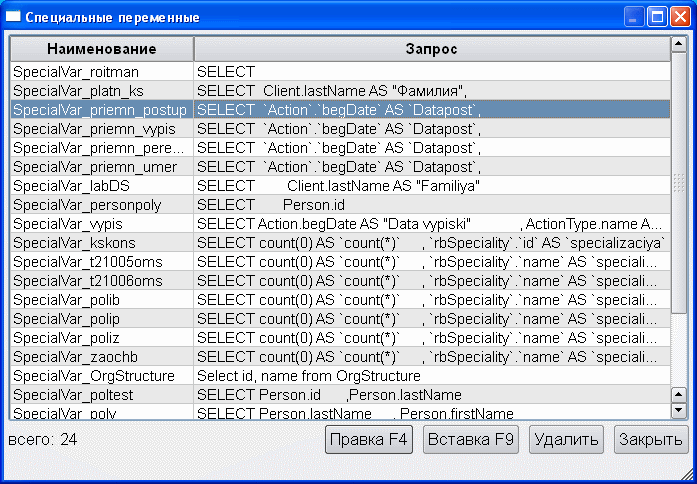
\includegraphics[width = 0.8\textwidth ,keepaspectratio]{patt_svar}
 \caption{Список специальных переменных}
 \label{img_patt_svar}
\end{figure}

\begin{figure}[ht]\centering
 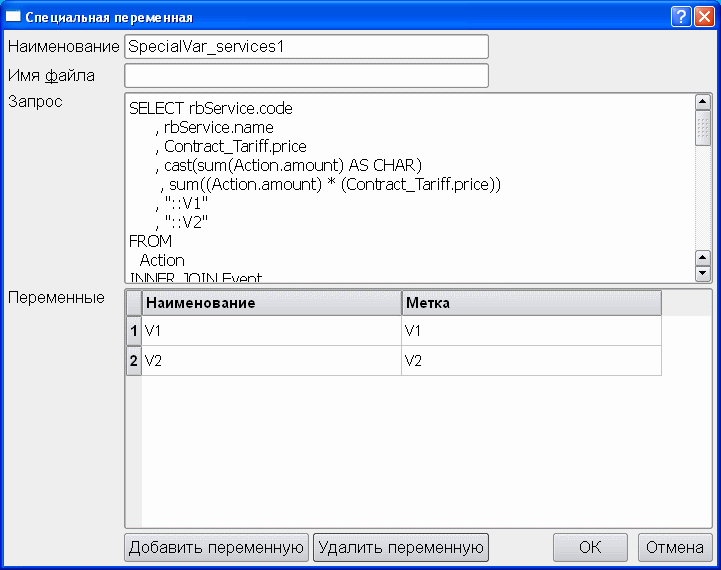
\includegraphics[width = 0.8\textwidth ,keepaspectratio]{patt_svar_card}
 \caption{Окно редактирования специальной переменной}
 \label{img_patt_svar_card}
\end{figure}

При добавлении новой специальной переменной необходимо указать (Рисунок \ref{img_patt_svar_card}):
\begin{itemize}
 \item \dm{Наименование переменной}. Оно должно быть уникально в списке специальных переменных и начинаться с префикса <<\code{SpecialVar\_}>>.
 \item \dm{Имя файла} – имя файла, содержащего SQL-запрос. Файл должен иметь расширение *.txt и располагаться в папке <<sqlqueries>> клиентского приложения.
 \item \dm{Запрос} – если имя файла в предыдущем поле не указано, то можно ввести текст SQL-запроса непосредственно в данное поле.
 \item \dm{Переменные}. Необходимо добавить в таблицу все переменные (параметры), участвующие в SQL-запросе, используя кнопки \btn{Добавить переменную} и  \btn{Удалить переменную}.
\end{itemize}

Текст SQL-запроса должен быть записан в след виде:

\verb|SELECT * FROM tablename where fio=::v1 and date=::v2;|

где \code{v1,v2} - переменные для SQL-запроса, значения которых указываются в тексте шаблона или вводятся с клавиатуры через механизм организации диалогов.

Для задания значений переменных, которые будут использоваться в SQL-запросе, в тексте шаблона необходимо использовать функцию \code{SpecialVariable()}. Первым аргументом функции нужно указать наименование переменной, а последующие переменные должны содержать значения всех переменных для SQL-запроса в том порядке, в котором они были описаны при создании специальной переменной.

Например, имеется специальная переменная \verb|SpecialVar_name1|, для которой заданы переменные \code{id} и \code{name}. Необходимо передать значение \code{id} равным 3 и значение \code{name} равным <<Name1>>. Для этого необходимо использовать конструкцию:

\verb|SpecialVariable('SpecialVar_name1', 3,'Name1')|

Для вывода на печать значения специальной переменной используется конструкция:
\begin{verbatim}

   
   {{i}}
   

\end{verbatim}

\subsection{Создание аналитических отчетов}

Для создания аналитического отчета необходимо:
\begin{itemize}
 \item Создать соответствующий шаблон печати в меню \mm{Настройки \str Шаблоны печати} (см. п. \ref{patt_add}) Как правило, при создании шаблонов печати для аналитических отчетов используются специальные переменные (см. п. \ref{patt_svar})
 \item Добавить аналитический отчет в меню  \dm{Настройки  \str Настройка свободных отчетов} (Рисунок \ref{img_patt_arep}). Добавление новых отчетов производится непосредственно в таблицу. Для этого нужно дважды щелкнуть левой кнопкой мыши в нижней (пустой) строке таблицы, активировав возможность ввода данных. В поле \dm{Наименование} нужно ввести с клавиатуры название отчета, как оно будет отображаться в меню, в поле \dm{Шаблоны печати} – выбрать из списка созданный на предыдущем шаге шаблон.
\end{itemize} 

\begin{figure}[ht]\centering
 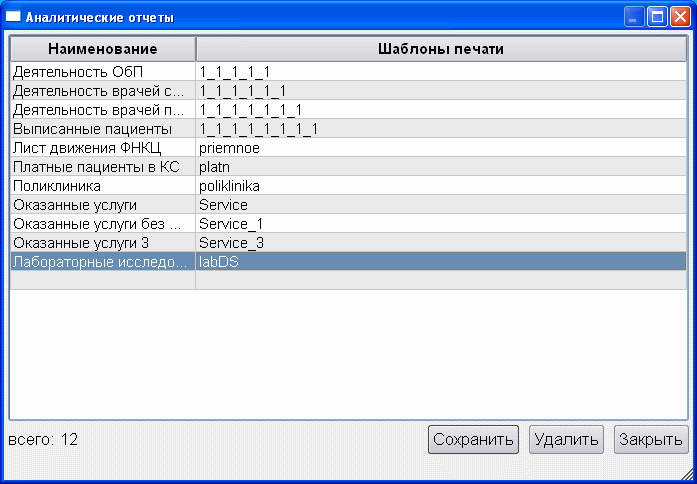
\includegraphics[width = 0.7\textwidth ,keepaspectratio]{patt_arep}
 \caption{Окно добавления аналитических отчетов}
 \label{img_patt_arep}
\end{figure}

После выполнения указанных действий в пункте меню \mm{Анализ \str Аналитические отчеты} появится отчет с указанным наименованием. %Создание шаблонов печатных форм
  \newpage
\section{Настройка прав и ролей пользователей }

Для обеспечения работы пользователей в системе необходимо настроить для них права доступа к определенным разделам \tmis~на выполнение определенных операций. Система разграничения доступа в \tmis~базируется на основе понятия ролей (профилей прав) пользователей.

В системе имеется список доступных полномочий (прав пользователей). Его можно вызвать из меню \mm{Настройки \str Права пользователей} (Рисунок \ref{img_acs_priv}). Код и назначение привилегий предопределяется разработчиками.

\begin{figure}[ht]\centering
 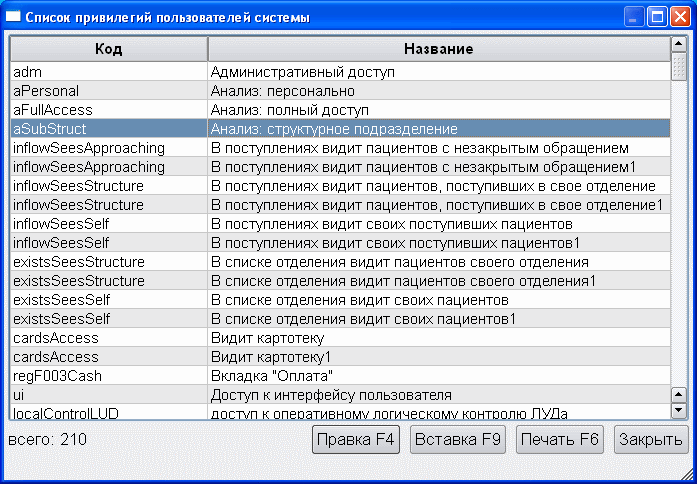
\includegraphics[width = 0.7\textwidth ,keepaspectratio]{acs_priv}
 \caption{Список привилегий пользователей}
 \label{img_acs_priv}
\end{figure}

Администратор системы должен создать для каждой группы пользователей набор привилегий. Такие наборы привилегии называются профилями прав или ролями пользователей. Они создаются из пункта меню \mm{Настройки \str Роли пользователей} (Рисунок \ref{img_acs_roles}).

Для добавления новой роли нужно нажать кнопку \btn{Вставка F9}, в открывшемся окне (Рисунок \ref{img_acs_role}) в поле \dm{Наименование} ввести название роли пользователя, отражающее ее суть (понятное для администратора системы), а в таблицу \dm{Разрешенные действия} добавить привилегии, необходимые для данной роли. Для добавления новой привилегии следует в нижней (пустой) строке дважды щелкнуть левой кнопкой мыши, активировав список привилегий, а затем выбрать нужную привилегию из списка. 

\begin{figure}[ht]\centering
 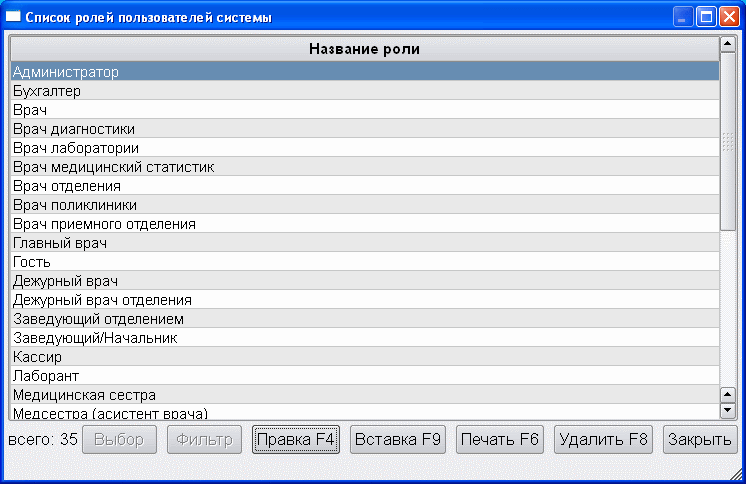
\includegraphics[width = 0.7\textwidth ,keepaspectratio]{acs_roles}
 \caption{Список ролей пользователей}
 \label{img_acs_roles}
\end{figure}

\begin{figure}[ht]\centering
 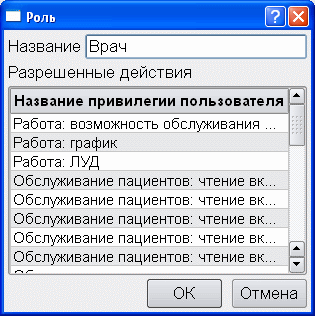
\includegraphics[width = 0.4\textwidth ,keepaspectratio]{acs_role}
 \caption{Настройка роли пользователя}
 \label{img_acs_role}
\end{figure}

Далее администратор может добавить пользователям созданную роль в справочнике \mm{Справочники \str Персонал \str Сотрудники}.

Для доступа к пункту меню \mm{Работа \str Обслуживание пациентов} у пользователя должна быть одна из следующих привилегий:
\begin{itemize}
 \item clientCardsAccess;
 \item clientRegRead;
 \item clientEventRead;
 \item clientInflowSeesSelf;
 \item clientInflowSeesStructure;
 \item clientInflowSeesApproaching;
 \item clientExistsSeesSelf;
 \item clientExistsSeesStructure.
\end{itemize}

Для работы с картотекой пациентов необходима привилегия <<cardsAccess>>, которая позволяет пользователю видеть картотеку пациентов.

Для работы с обращениями у пользователя должны быть некоторое из перечисленных в таблице \ref{tbl_acs_priv_obr} привилегий.

{\small
\begin{longtable}{|p{4cm}|p{5cm}|p{7.7cm}|}
\caption{Список привилегий для работы с обращениями \label{tbl_acs_priv_obr}} \\
\hline \rule{0pt}{15pt} \centering \textbf{Код права} & \centering \textbf{Название} & \hfil \textbf{Описание} \\ \hline
\endfirsthead
\hline \rule{0pt}{15pt} \centering \textbf{Код права} & \centering \textbf{Название} & \hfil \textbf{Описание} \\ \hline
\endhead
 clientEventCreate & 	Пациенты: обращения, создание &	Необходимо для создания новых обращений \\ \hline
 clientEventRead &	Пациенты: Обращения, чтение &	Делает доступным пункт меню \mm{Работа \str Обслуживание пациентов}, предоставляет возможность просмотра обращений \\ \hline
 clientEventUpdate &	Пациенты: обращения, изменение & 	Предоставляет возможность редактирования обращений \\ \hline
 changeExecPerson &	Имеет возможность изменять лечащего врача в обращении &	Так же пользователь может менять ответственного, если он создал это обращение \\ \hline
 changeFinanceSource & Имеет возможность изменять источники финансирования &	Для стационарных обращений \\ \hline
 evtEditClosed & Имеет возможность редактировать закрытые обращения &  \\ \hline
 evtDelAll & Имеет возможность удалять любое обращение &  \\ \hline 	
 evtDelOwn &	Имеет возможность удалять только свои обращения &	Свое обращение – это то, где пользователь является ответственным либо обращения, которые были созданы пользователем и не редактировались другими участниками системы \\ \hline
\end{longtable}
}

Для работы с действиями пользователю могут потребоваться следующие привилегии (Таблица \ref{tbl_acs_priv_act}):

\begin{table}[h]
\small
\topcaption{Привилегии для работы с действиями} \label{tbl_acs_priv_act} 
 \begin{tabular}{|p{3.8cm}|p{5cm}|p{7.9cm}|}
  \hline \rule{0pt}{15pt} \centering \textbf{Код права} & \centering \textbf{Название} & \hfil \textbf{Описание} \\ \hline
  copyPrevAction &	Копировать действия из предыдущих событий &	Делает доступной кнопку \btn{Копировать из предыдущего}  при редактировании действия \\ \hline
  loadActionTemplate &	Применять шаблоны действий &	Делает доступной кнопку  \btn{Загрузить шаблон}  при редактировании действия \\ \hline
  richEditor & Видеть кнопку редактора & \\ \hline
 \end{tabular}
\end{table}

Для того чтобы пользователь имел возможность записи пациентов на прием, необходимо, чтобы у него была одна из следующих привилегий(Таблица \ref{tbl_acs_priv_reg}):

\begin{table}[h]
\small
\topcaption{Привилегии для записи на прием} \label{tbl_acs_priv_reg} 
 \begin{tabular}{|p{3.5cm}|p{5.9cm}|p{7.3cm}|}
  \hline \rule{0pt}{15pt} \centering \textbf{Код права} & \centering \textbf{Название} & \hfil \textbf{Описание} \\ \hline
  enquePrimary &	Может записывать как регистратор &	Запись по квотам <<Запись из регистратуры>> \\ \hline
  enqueOwn  &	Имеет возможность поставить в очередь как врач, записывающий пациента к себе на повторный прием &	Данная роль должна выдаваться врачам, ведущим амбулаторный прием. Запись по квотам <<Запись врачом на повторный прием>> \\ \hline
  enqueConsultancy	& Имеет возможность поставить в очередь как врач, записывающий пациента к другому врачу &	Запись по квотам <<Межкабинетная запись>> \\ \hline
 \end{tabular}
\end{table}

Для работы с листами назначений могут потребоваться некоторые из привилегий, приведенных в таблице \ref{tbl_acs_priv_ln}. \index{Листы назначений (настройки)}

{\small
\begin{longtable}{|p{4.2cm}|p{5cm}|p{7.5cm}|}
\caption{Привилегии для работы с листами назначений \label{tbl_acs_priv_ln}} \\
\hline \rule{0pt}{15pt} \centering \textbf{Код права} & \centering \textbf{Название} & \hfil \textbf{Описание} \\ \hline
\endfirsthead
\hline \rule{0pt}{15pt} \centering \textbf{Код права} & \centering \textbf{Название} & \hfil \textbf{Описание} \\ \hline
\endhead
clientPrescriptionsRead &	Имеет возможность просматривать и печатать лист назначений &	Возможность просмотра и печати листа назначений из карточки обращения \\ \hline
clientPrescriptions CreateOwn &	Имеет возможность создавать новые назначения только в тех обращениях, где пользователь является ответственным	& Делает доступной кнопку \btn{Создать назначение}  в листе назначений в карточках тех обращений, где текущий пользователь является ответственным  \\ \hline
clientPrescriptions CreateAll &	Имеет возможность создавать новые назначения во всех обращениях	& Делает доступной кнопку   \btn{Создать назначение}  в листе назначений в карточках всех обращений \\ \hline
clientPrescriptions EditOwn	& Имеет возможность редактировать, отменять назначения только в тех обращениях, где пользователь является ответственным	& Делает доступной для редактирования карточки ранее созданных назначений в листе назначений карточек обращений, где пользователь является ответственным  \\ \hline
clientPrescriptions EditAll	& Имеет возможность редактировать, отменять назначения во всех обращениях & 	Делает доступной для редактирования карточки ранее созданных назначений в листе назначений всех карточек обращений \\ \hline
wJobsOperating	& Имеет доступ к форме листа исполнений & Форма \dm{Лист назначений (исполнения)} является доступной для использования \\ \hline
clientPrescriptionsExec EditOwn	& Имеет возможность исполнять назначения только в рамках своего отделения  ЛПУ	& Форма \dm{Лист назначений (исполнения)} является доступной для использования, пользователь не имеет возможности изменения значения поля \dm{Подразделение}. В поле \dm{Подразделение} указано подразделение пользователя \\ \hline
clientPrescriptionsExec EditAll	& Имеет возможность исполнять назначения во всех отделениях ЛПУ	& Форма \dm{Лист назначений (исполнения)} является доступной для использования, имеется возможность выбора подразделения \\ \hline
clientPrescriptionsExec ChangeOrgStruct & Имеет возможность просматривать исполнения назначений в любом отделении ЛПУ в форме листа исполнений	& Форма \dm{Лист назначений (исполнения)} является доступной для просмотра исполнений и печати листа назначений, имеется возможность выбора подразделения \\ \hline
\end{longtable}
}

Рекомендуемые настройки прав пользователей по листам назначений приведены в таблице \ref{tbl_acs_roles_ln}.

{\small
\begin{longtable}{|p{7.6cm}|p{2.1cm}|p{2.1cm}|p{2.1cm}|p{2.1cm}|}
\caption{Рекомендуемые настройки прав пользователей \label{tbl_acs_roles_ln}} \\
\hline \rule{0pt}{15pt} \centering \textbf{Код права} & \centering \textbf{Врач отделения} & \centering \textbf{Дежур\-ный врач} & \centering \textbf{Медсест\-ра отделения} & \textbf{Админист\-ра\-ция ЛПУ} \\ \hline
\endfirsthead
\hline \rule{0pt}{15pt} \centering \textbf{Код права} & \centering \textbf{Врач отделения} & \centering \textbf{Дежур\-ный врач} & \centering \textbf{Медсест\-ра отделения} & \textbf{Адми\-нист\-ра\-ция ЛПУ} \\ \hline
\endhead			
clientPrescriptionsRead &	\centering $+$	&	\centering $+$		&	\centering $+$ & \hfil $+$ \\ \hline
clientPrescriptionsCreateOwn &		\centering $+$	& & & \\ \hline		
clientPrescriptionsCreateAll & &	\centering $+$ & & \\ \hline		
clientPrescriptionsEditOwn	&	\centering $+$ & & & \\ \hline			
clientPrescriptionsEditAll	&	&	\centering $+$ & & \\ \hline		
wJobsOperating	& &	 & 	\centering $+$	& \hfil $+$ \\ \hline
clientPrescriptionsExecEditOwn & & & \centering $+$ & \\ \hline	
clientPrescriptionsExecEditAll	& & & & \\ \hline			
clientPrescriptionsExecChangeOrgStruct	& & & & \hfil $+$ \\ \hline
\end{longtable}
}

\subsection{Настройка доступных типов действий для пользователей и ролей}

В системе существует возможность ограничить список типов действий, которые видит пользователь при создании очередной медицинской записи в карточке обращения, т.е. можно наложить фильтр на доступные типы действий. Возможна настройка ограничений для определенной роли или конкретного пользователя.

Для настройки фильтрации типов действий необходимо выбрать пункт меню \mm{Настройки \str Фильтр типов действий}. Откроется форма (Рисунок \ref{img_acs_tpact_filtr}) \dm{Фильтры типов действий}. В левой ее части находятся 2 вкладки. На вкладке \dm{Пользователи} настраиваются доступные типы действий для конкретных пользователей. На вкладке \dm{Роли} настраиваются доступные типы действий для всех пользователей, работающих под указанной ролью.

\begin{figure}[ht]\centering
 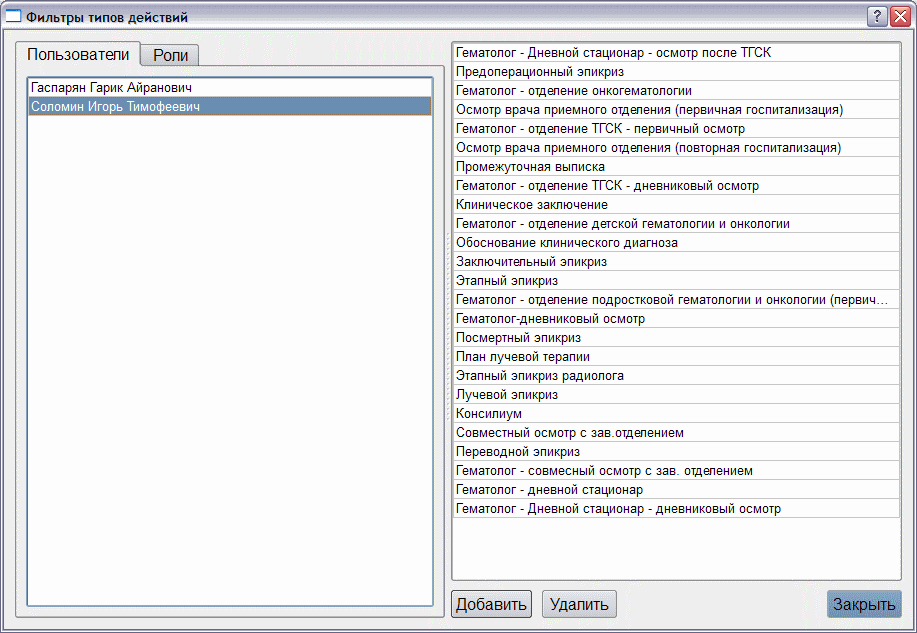
\includegraphics[width = 0.8\textwidth ,keepaspectratio]{acs_tpact_filtr}
 \caption{Форма настройки фильтраций типов действий для пользователей}
 \label{img_acs_tpact_filtr}
\end{figure}

\subsubsection{Создание нового правила фильтрации} \label{acs_tpactfiltr}

Для того чтобы создать новое правило фильтрации типов действий для пользователя или роли нужно перейти на соответствующую вкладку и нажать кнопку \btn{Добавить} в правом нижнем углу формы. Откроется новая форма \dm{Создание действий} (Рисунок \ref{img_acs_tpact_filtradd}). В левом верхнем углу, в поле со списком (второе сверху) в зависимости от вида создаваемого правила, следует выбрать фамилию пользователя или название роли. Далее, необходимо в таблицу \dm{Выбранные действия}, расположенную в правой части формы добавить типы действий, которые будут доступны указанному пользователю/роли. Добавление новых типов действий производится двойным щелчком мыши либо перетаскиванием (drag\&drop) соответствующего наименования типа действия из левой части формы в правую. В левой части может быть использовано как представление в виде списка, так и в виде дерева.

После того как список типов действий в таблице \dm{Выбранные действия} сформирован, необходимо нажать кнопку \btn{OK}  в правом нижнем углу формы. Текущая форма закроется, а в форме \dm{Фильтры типов действий} появится новая запись на активной вкладке.

\begin{figure}[ht]\centering
 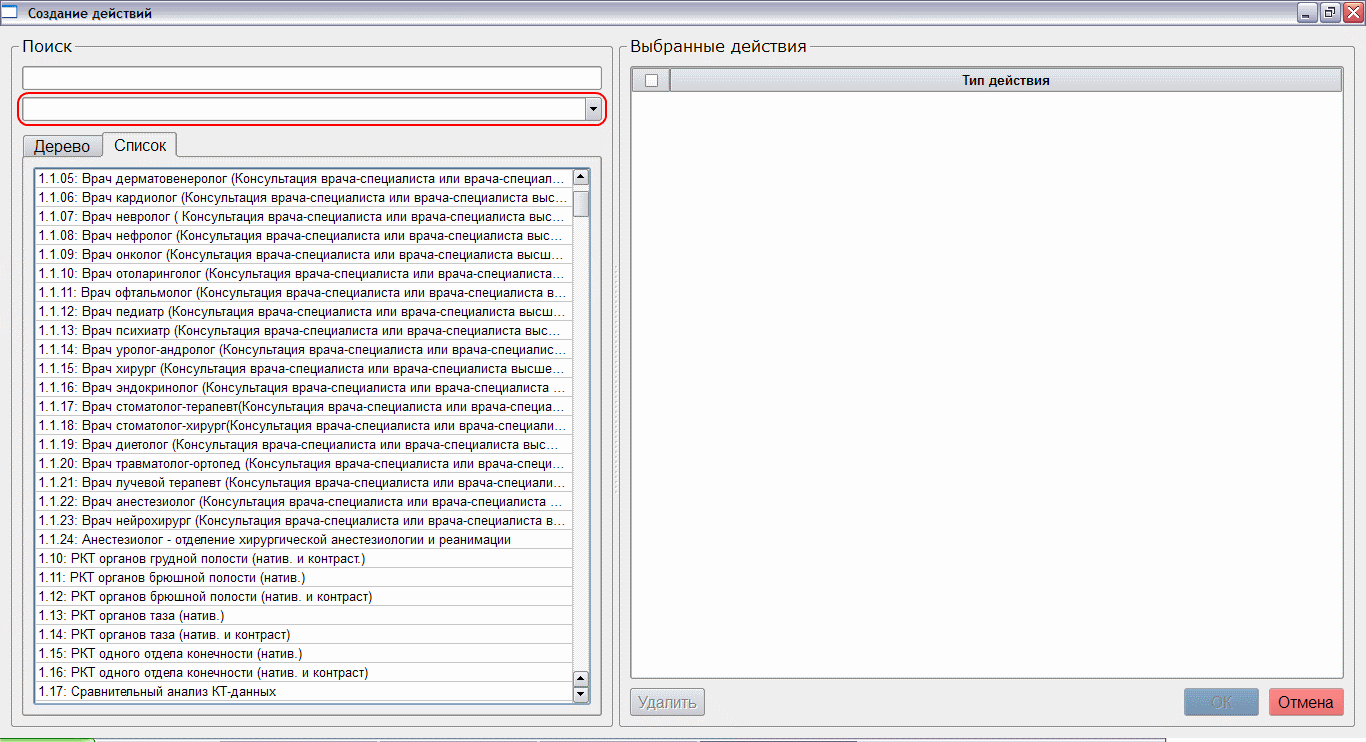
\includegraphics[width = 1\textwidth ,keepaspectratio]{acs_tpact_filtradd}
 \caption{Добавление правил фильтрации типов действий}
 \label{img_acs_tpact_filtradd}
\end{figure}

\subsubsection{Просмотр правила фильтрации}

Для того чтобы просмотреть список доступных типов действий для пользователя или роли, необходимо перейти на соответствующую вкладку (\dm{Пользователи} или \dm{Роли}) и установить курсор на определенной фамилии пользователя или названии роли, щелкнув по ней левой кнопкой мыши. После этого в правой части формы появится список доступных типов действий для выбранного пользователя\slash роли.

\subsubsection{Редактирование правил фильтрации}

Для редактирования списка доступных типов действий следует дважды щелкнуть левой кнопкой мыши по фамилии соответствующего пользователя или наименованию роли. Откроется форма \dm{Создание действий} (Рисунок \ref{img_acs_tpact_filtradd}), содержащее настройки фильтрации типов действий для выбранного пользователя\slash роли. Можно добавить или удалить типы действий из списка \dm{Выбранные действия}.

Добавление новых типов действий подробно описано в подразделе \ref{acs_tpactfiltr}

Для удаления наименования типа действия из списка следует установить напротив него флаг  \putx~и нажать кнопку  \btn{Удалить} в правой нижней части формы. Для удаления наименований нескольких типов действий одновременно можно установить флажки   напротив их наименований, а затем нажать кнопку \btn{Удалить}.

После того как все изменения внесены в правило фильтрации следует нажать кнопку  \btn{OK} в правом нижнем углу формы. Будет осуществлен возврат к форме \dm{Фильтры типов действий}.

Для удаления правила фильтрации необходимо установить курсор на соответствующей фамилии пользователя или названии роли в левой части формы (Рисунок \ref{img_acs_tpact_filtr}) и нажать кнопку  \btn{Удалить} в правой нижней части формы.

\subsubsection{Порядок фильтрации типов действий}

При фильтрации типов действий установлен следующий порядок:
\begin{itemize}
 \item Если для текущего пользователя \textbf{не задано} правило фильтрации \textbf{по имени пользователя} и \textbf{не задано} правило фильтрации \textbf{по роли}, то при создании новой медицинской записи он может видеть \textbf{все типы действий}.
 \item Если для текущего пользователя \textbf{не задано} правило фильтрации \textbf{по имени пользователя}, но \textbf{задано} правило фильтрации \textbf{по роли}, то при создании новой медицинской записи он может видеть только  типы действий, определенные \textbf{для его роли}.
 \item Если для текущего пользователя \textbf{задано} правило фильтрации \textbf{по имени пользователя}, но \textbf{не задано} правило фильтрации \textbf{по роли}, то при создании новой медицинской записи он может видеть только типы действий, определенные \textbf{для данного пользователя}.
 \item Если для текущего пользователя \textbf{задано} правило фильтрации \textbf{по имени пользователя} и \textbf{задано} правило фильтрации \textbf{по роли}, то при создании новой медицинской записи он может видеть только типы действий, определенные \textbf{для данного пользователя}.
\end{itemize}
 
 %Настройка прав и ролей пользователей 
  \newpage
\section{Прочие настройки}

\subsection{Настройка фонового изображения и логотипа}

Настройка фонового изображения и логотипа возможна только при входе пользователя под ролью <<Администратор>>.

Настройка выполняется в меню \mm{Настройки \str Внешний вид} на вкладке \dm{Администратор} (Рисунок \ref{img_oth_vid}) (она становится доступна только под администратором).

\begin{figure}[ht]\centering
 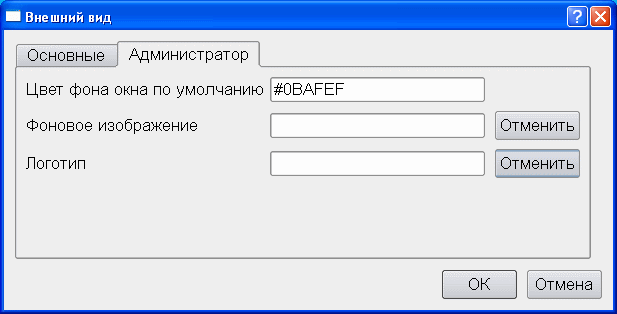
\includegraphics[width = 0.6\textwidth ,keepaspectratio]{oth_vid}
 \caption{Настройка внешнего вида}
 \label{img_oth_vid}
\end{figure}

Для изменения цвета фона окна следует щелкнуть левой кнопкой мыши по полю \dm{Цвет фона окна по умолчанию} и в открывшемся окне подобрать цвет и нажать кнопку \btn{OK}.

Для добавления фонового изображения в окно программы нужно щелкнуть левой кнопкой мыши в поле \dm{Фоновое изображение}, указать путь к файлу изображения и нажать кнопку  \btn{Открыть}. После чего файл будет загружен в БД. Размер загружаемого файла не должен превышать 250 Кб. Аналогичным образом загружается логотип в поле \dm{Логотип}. Рекомендуемый размер логотипа – не более 100х100 пискелей.

\subsection{Настройка соединений с внешними системами}

\subsubsection{Система журналирования}

Система журналирования – это внешний модуль, подключение которого позволяет вести лог следующих действий в \tmis:
\begin{itemize}
 \item Авторизация пользователя в системе;
 \item Печать документа;
 \item Тип действия: создание, удаление, изменение;
 \item Событие: создание, удаление, изменение;
 \item Действие: создание, удаление, изменение;
 \item Ошибки, связанные с ошибками работы, обращениями в БД.
\end{itemize}
 
Для включения или отключения системы журналирования в \tmis~следует выбрать пункт \mm{Настройки \str Настройки \tmis}. В открывшейся форме слева, в группе <<Подсистемы \tmis>>, нужно выбрать пункт \dm{Система журналирования} двойным щелчком левой кнопки мыши (Рисунок \ref{img_oth_jur}).

\begin{figure}[ht]\centering
 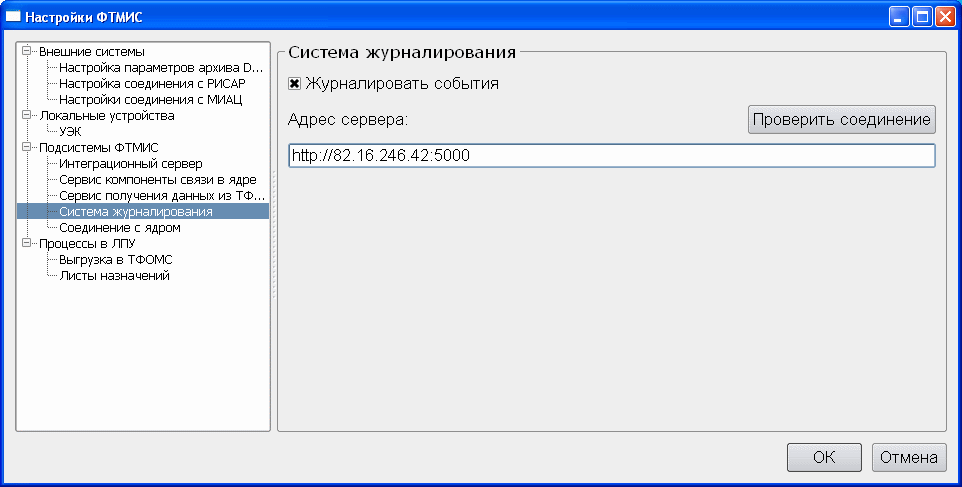
\includegraphics[width = 0.8\textwidth ,keepaspectratio]{oth_jur}
 \caption{Настройка системы журналирования}
 \label{img_oth_jur}
\end{figure}

Для ведения лога перечисленных выше событий необходимо установить флаг \dm{Журналировать события} и в строке \dm{Адрес сервера} указать адрес и порт сервера, по которым доступна система журналирования. После указания адреса рекомендуется выполнить проверку наличия соединения с системой журналирования, нажав кнопку \btn{Проверить соединение} . В случае успешного соединения, на экране появится сообщение (Рисунок \ref{img_oth_jur_con}). В случае получения сообщения об ошибке соединения, следует исправить адрес и выполнить проверку снова.

\begin{figure}[ht]\centering
 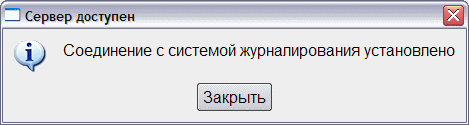
\includegraphics[width = 0.5\textwidth ,keepaspectratio]{oth_jur_con}
 \caption{Сообщение об успешном соединении с сервером журналирования}
 \label{img_oth_jur_con}
\end{figure}

\begin{vnim}
Сохранение флага включения системы журналирования возможно только после выполнения проверки соединения с сервером
\end{vnim}

Для того чтобы настройки вступили в силу, нужно сохранить их, нажав кнопку  \btn{OK} в правом нижнем углу формы.

Для отключения ведения лога событий следует снять флаг \dm{Журналировать события} и нажать кнопку \btn{OK} в правом нижнем углу формы.

\subsubsection{Листы назначений} \index{Листы назначений (настройки)}

Для доступа к настройкам листов назначений необходимо в главном меню выбрать пункт \mm{Настройки \str Настройки \tmis}. В открывшемся окне слева, в группе <<Процессы в ЛПУ>>, выбрать пункт \dm{Листы назначений} двойным щелчком левой кнопки мыши. При этом в правой части окна появятся настройки (Рисунок \ref{img_oth_ln}).

\begin{figure}[ht]\centering
 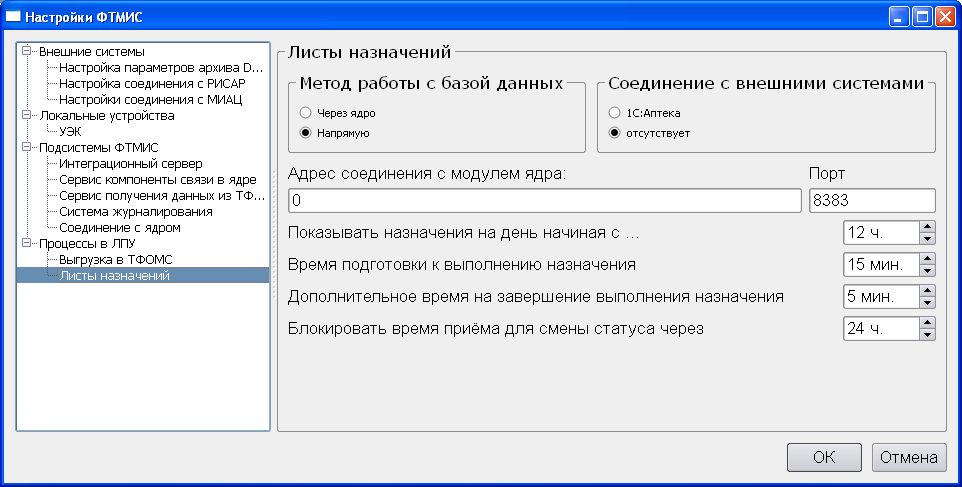
\includegraphics[width = 0.8\textwidth ,keepaspectratio]{oth_ln}
 \caption{Настройка листов назначений}
 \label{img_oth_ln}
\end{figure}

Для организации работы с листами назначений имеются следующие настройки:
\begin{itemize}
 \item \dm{Метод работы с базой данных} определяет способ взаимодействия с ядром. Следует всегда выбирать значение <<Напрямую>>.
 \item \dm{Соединение с внешними системами}: на текущий момент поддерживается только взаимодействие с системой <<1С:Аптека>>. Если в данном пункте выбрано значение <<1С: Аптека>>, то
 \begin{itemize}
  \item движение пациентов в стационаре будет передаваться в <<1С:Аптека>>;
  \item из <<1С:Аптека>> будет запрошен справочник медикаментов (РЛС);
  \item при поиске препаратов для добавления в лист назначений пациента будет производиться запрос остатков по препаратам найденной группы в <<1С:Аптека>>;
  \item будет выполняться полное обновление остатков по препаратам 1 раз в сутки (в 1:30).
 \end{itemize} 
 \item \dm{Адрес соединения с модулем ядра} необходимо указать, только в случае, если осуществляется взаимодействие с <<1С:Аптека>>. В данной строке указывается IP-адрес сервера размещения ядра.
 \item \dm{Порт} соединения с модулем ядра необходим только в случае, если осуществляется взаимодействие с <<1С:Аптека>>.
 \item \dm{Показывать назначения на день начиная с} определяет час суток, начиная с которого выполняется графление суточного листа назначений в системе Рекомендуемое значение – 12 часов.
 \item \dm{Время подготовки к выполнению назначения} определяет за сколько минут до наступления времени приема препарата оно переходит в состояние «Выполняется» (время на приготовление препарата). Рекомендуемое значение – 15 минут.
 \item \dm{Дополнительное время на завершение выполнения назначения} определяет количество минут, на сколько задерживается переход из состояния «Выполняется» после завершения интервала приема препарата. Рекомендуемое значение – 5 минут.
 \item \dm{Блокировать время приема для смены статуса через} определяет время, в течении которого можно поставить отметку о выполнении либо отменить назначение, после завершения времени приема препарата. По истечении указанного времени от момента окончания назначенного времени приема препарата, он становится недоступным для редактирования. Рекомендуемое значение – 24 часа.
\end{itemize} 

\subsubsection{Настройки для выгрузки в ТФОМС}

Для настройки обязательности некоторых полей, необходимых для выгрузки в ТФОМС необходимо выбрать пункт \mm{Настройки \str Настройки \tmis}. В открывшейся форме слева, в группе <<Процессы в ЛПУ>>, нужно выбрать пункт \dm{Выгрузка в ТФОМС} двойным щелчком левой кнопки мыши (Рисунок \ref{img_oth_tfoms}).

\begin{figure}[ht]\centering
 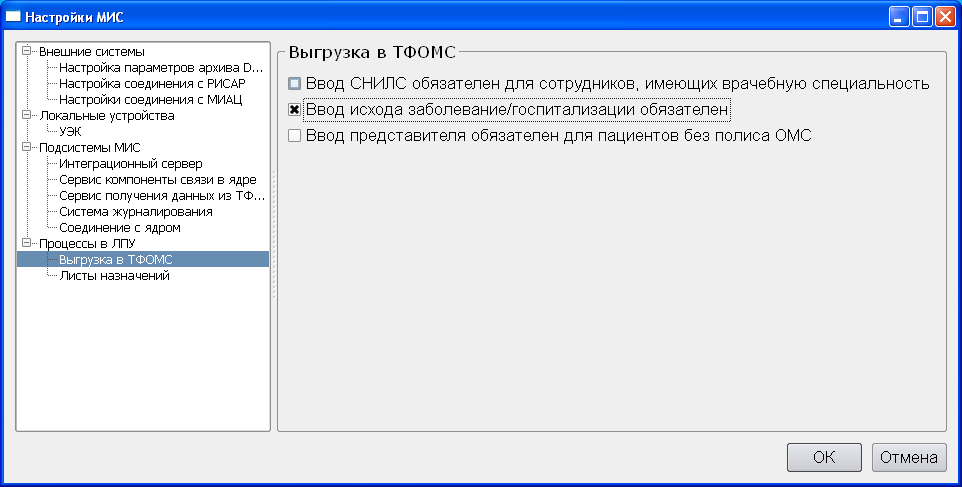
\includegraphics[width = 0.8\textwidth ,keepaspectratio]{oth_tfoms}
 \caption{Настройка обязательности некоторых полей}
 \label{img_oth_tfoms}
\end{figure}

В данном разделе можно настроить обязательность заполнения следующих полей:
\begin{itemize}
 \item \dm{Ввод СНИЛС обязателен для сотрудников, имеющих врачебную специальность} -- настройка обязательности заполнения поля СНИЛС для врачей в справочнике сотрудников (\mm{Справочники \str Персонал \str Сотрудники});
 \item \dm{Ввод исхода заболевания\slash госпитализации обязателен} -- настройка обязательности заполнения поля \dm{Исход}  в карточке обращения;
 \item \dm{Ввод представителя обязателен для пациентов без полиса ОМС} -- при установке данного флажка становится обязательным добавление представителя на вкладку \dm{Связи} регистрационной карточки пациента в случае, если не введены данные полиса ОМС данного пациента.
\end{itemize}

Для того чтобы настройки вступили в силу, нужно сохранить их, нажав кнопку  \btn{OK} в правом нижнем углу формы. 

\subsection{Настройка счетчиков}

Для многих событий, регистрируемых в \tmis, требуется вести отдельную нумерацию. Например, должен вестись отдельный учет поликлинических и стационарных обращений. Формат номеров обращений и механизм учета (в частности, номеров историй болезни) утвержден и используется уже очень давно. Чтобы не ломать привычный механизм работы в ЛПУ, \tmis~позволяет вести нумерацию событий с помощью гибко настраиваемого механизма счетчиков.

Порядок работы со счетчиками следующий:
\begin{enumerate}
 \item В пункте меню \mm{Настройки \str Счетчики} регистрируется и настраивается новый счетчик (см. ниже).
 \item В справочнике \dm{Типов событий} (\mm{Справочники \str Учет \str Типы событий}) организуется связь с данным счетчиком. Для этого на вкладке \dm{Основная информация} следует установить флажок \dm{Требуется ввод внешнего идентификатора} и в поле \dm{Счетчик} выбрать созданный в п. 1 тип счетчика.
\end{enumerate}

После выполнения указанных настроек всем событиям данного типа будут присваиваться внешние идентификаторы в соответствии с настройками нового счетчика.

\begin{figure}[ht]\centering
 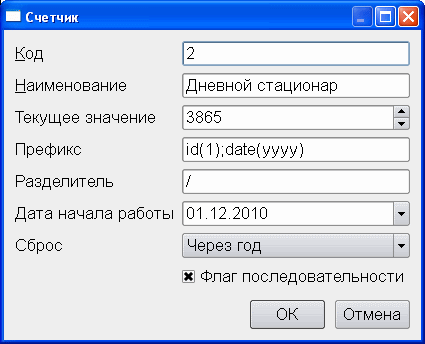
\includegraphics[width = 0.5\textwidth ,keepaspectratio]{oth_cnt}
 \caption{Карточка редактирования счетчика}
 \label{img_oth_cnt}
\end{figure}

При создании счетчика в пункте меню \mm{Настройки \str Счетчики} необходимо выполнить следующие настройки (Рисунок \ref{img_oth_cnt}):
\begin{itemize}
 \item \dm{Код} – уникальный код счетчика;
 \item \dm{Наименование} – наименование счетчика, отражающее его назначение;
 \item \dm{Текущее значение} – при создании счетчика следует указать начальное значение создаваемого счетчика. В дальнейшем, при создании событий, связанных с данным счетчиком, значение поля будет меняться автоматически. Изменять его вручную не рекомендуется.
 \item \dm{Префикс} – Номер события может быть составным. В начале указывается некоторый префикс, например, номер года для историй болезни, а затем, через разделитель, собственно номер события. Префикс может содержать несколько значений. В этом случае все они будут отображаться через разделитель. Пустые префиксы не отображаются. Например, если в поле префикс указано <<id(1);date(yyyy)>>, то номер события будет иметь формат <идентификатор пациента>/<номер года>/<текущее значение счетчика>, где <идентификатор пациента> – это идентификатор пациента во внешней системе с кодом <<1>> (раздел \ref{oth_outsys}). Если данный идентификатор у пациента отсутствует, то номер события будет иметь формат <номер года>/<текущее значение счетчика>.
 \item \dm{Разделитель} – символ разделителя, устанавливаемый между префиксом и основным номером;
 \item \dm{Дата начала работы} – устанавливается автоматически при создании счетчика;
 \item \dm{Сброс} – периодичность обнуления счетчика. Например, нумерация историй болезни пациентов начинается заново каждый год, поэтому для событий данного типа следует устанавливать значение поля \dm{Сброс} = <<Через год>>;
 \item При установке флажка \dm{Флаг последовательности} будут использоваться последовательные уникальные номера.
\end{itemize}

\subsection{Настройка выходных и праздничных дней}

При работе \tmis~используется стандартный календарь. Выходными днями считаются суббота и воскресенье. Национальные праздники не учитываются в стандартном календаре. Однако, в системе существует возможность настройки праздничных дней и переносов выходных дней. При добавлении праздничного дня или переноса выходного дня он будет отображаться красным цветом в календаре, но при составлении расписания такие выходные дни не учитываются.

Для выполнения настроек выходных и праздничных дней следует выбрать пункт меню \mm{Настройки \str Календарь}. В открывшемся окне (Рисунок \ref{img_oth_hol}) на вкладке \dm{Праздники} следует ввести все праздничные дни в году. Праздники будут автоматически распространяться на все последующие годы. Если какой-либо праздник вводится вновь или отменяется, рекомендуется использовать поля указания года начала и\slash или окончания праздника совместно с флажками \dm{Есть год начала} и\slash или \dm{Есть год окончания} соответственно.
 
\begin{figure}[ht]\centering
 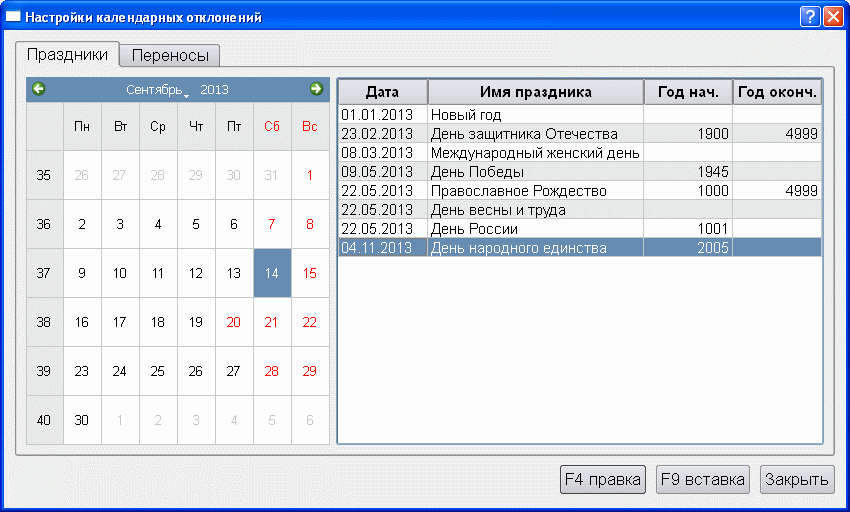
\includegraphics[width = 0.6\textwidth ,keepaspectratio]{oth_hol}
 \caption{Настройка праздничных дней}
 \label{img_oth_hol}
\end{figure}

На вкладке \dm{Переносы} можно настроить переносы выходных дней в связи с тем, что праздники выпадают на выходные. Настройка относится только к определенной дате указанного года и не распространяется на последующие годы. В поле \dm{Дата} (Рисунок \ref{img_oth_hol_per}) следует указать дату, которая становится выходным днем в связи с переносом, в поле \dm{Дата переноса} ввести исходную праздничную дату, которая выпала на выходной.

\begin{figure}[ht]\centering
 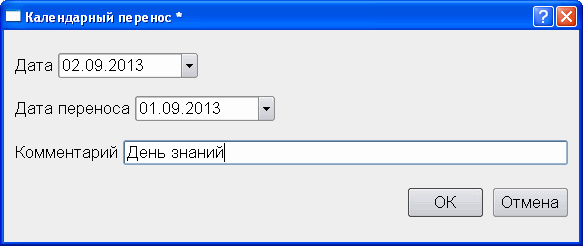
\includegraphics[width = 0.6\textwidth ,keepaspectratio]{oth_hol_per}
 \caption{Настройка переносов выходных дней}
 \label{img_oth_hol_per}
\end{figure}

\subsection{Создание правил для записи на прием}

В \tmis~возможно организовать квотирование записи пациентов на прием по времени или количеству пациентов. Настройки квотирования по времени выполняются в окне редактирования расписания сотрудника (\mm{Работа \str Учет рабочего времени}). Настройка квотирования по количеству пациентов выполняется в карточке сотрудника (\mm{Справочники \str Персонал \str Сотрудники}). При использовании метода квотирования по времени, в случае если часть талонов по какой-либо квоте остается неиспользованной, можно настроить автоматический переход неиспользованных талонов в другой тип за день или в день приема.

Настройка производится в пункте меню \mm{Настройки \str Правила записи на прием} (Рисунок \ref{img_oth_rule_per}). Редактирование и добавление записей нужно производить прямо в таблицу на форме, указав следующие данные:
\begin{itemize}
 \item \dm{Вид записи, из которого переходят талоны} (выбирается из списка);
 \item \dm{Вид записи, в который переходит талоны} (выбирается из списка);
 \item \dm{День перехода} (выбирается из списка). Можно выбрать значение <<За день до приема>> или <<В день приема>>;
 \item \dm{Время перехода} – время суток, в которое будет осуществлен переход. По умолчанию устанавливается время <<00:00>>;
 \item При установке флажка \dm{Талоны доступны для исходного вида записи}, будет возможна запись как по старой, так и по новой квоте. Если флажок не установлен, то после перехода будут доступны талоны только по новой квоте.
\end{itemize}

\begin{figure}[ht]\centering
 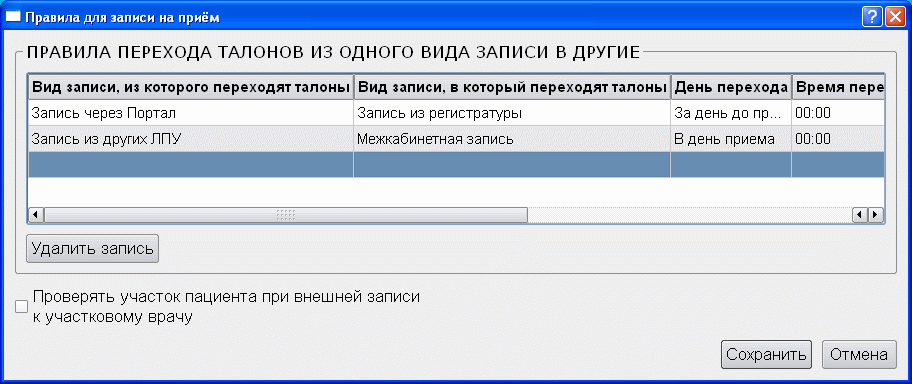
\includegraphics[width = 0.8\textwidth ,keepaspectratio]{oth_rule_per}
 \caption{Настройка правил перехода талонов}
 \label{img_oth_rule_per}
\end{figure}

\subsection{Внешние учетные системы} \label{oth_outsys}

В \tmis~существует возможность хранения идентификаторов пациентов в других информационных системах, что позволяет идентифицировать пациента и организовать получение и передачу данных пациентов в различные системы. Ввод и редактирование идентификаторов пациента во внешних системах производится в карточке пациента на вкладке \dm{Идентификаторы}.

Типы внешних систем, идентификаторы которых могут храниться в карточке пользователя, настраиваются в пункте меню \mm{Настройки \str Внешние учетные системы} (Рисунок \ref{img_oth_outsys}). Для пациента может быть сохранен только один идентификатор каждого типа, но количество типов идентификаторов при этом не ограничено и определяется только настройками справочника.

\begin{figure}[ht]\centering
 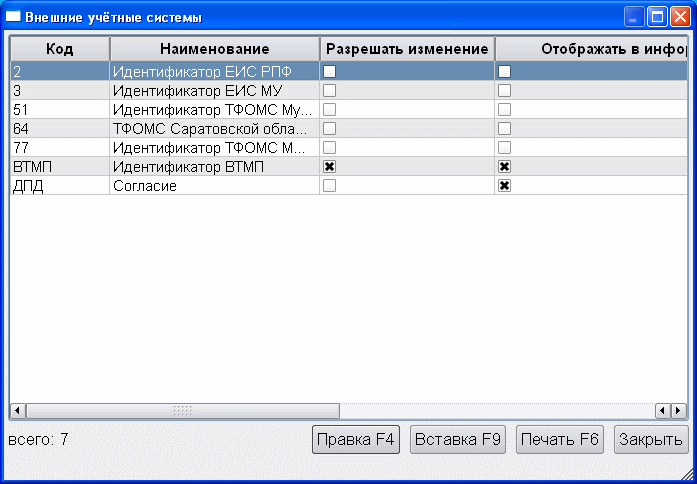
\includegraphics[width = 0.8\textwidth ,keepaspectratio]{oth_outsys}
 \caption{Справочник внешних учетных систем}
 \label{img_oth_outsys}
\end{figure}

\dm{Код} типа идентификатора должен быть уникальным, в поле \dm{Наименование} вводится название идентификатора, которое будет отображаться в карточках пациентов и фильтрах системы. Если флаг \dm{Разрешить изменение} не установлен, то редактирование ранее введенных идентификаторов невозможно.

\subsection{Настройка обмена с ТФОМС}

Настройки форматов обмена с ТФОМС производятся в отдельной системе~– Системе администрирования ЛПУ.

\subsection{Сообщения информатора}

В пункте меню \mm{Настройки \str Сообщения информатора} администратор системы может отправить \opr{всем} пользователям информационные сообщения. Сообщения будет выведено на экран пользователя при следующем входе в систему. Так же пользователь может просмотреть сообщения из пункта меню \mm{Сессия \str Информатор}.

\subsection{Настройки, выполняемые непосредственно В БД}

\subsubsection{Настройки, необходимые для работы листов назначений} \index{Листы назначений (настройки)}

\paragraph{Настройки складов для учета наличия медикаментов}

\begin{vnim}
 Данная настройка требуется только если организовано взаимо\-дей\-ствие с <<1С:Аптека>>
\end{vnim}
 
На данный момент настройку складов можно производить только непосредственно в таблице \code{rbStorage} базы данных. Структура таблицы приведена ниже.

\begin{table}
\small
\topcaption{Структура таблицы rbStorage} \label{tbl_oth_rbstor} 
 \begin{tabular}{|p{4cm}|p{4cm}|p{8.7cm}|}
  \hline \rule{0pt}{15pt} \centering \textbf{Поле} & \centering \textbf{Тип данных} & \hfil \textbf{Краткое описание} \\ \hline
  id &	INT &	Идентификатор  \\ \hline
  uuid &	VARCHAR(50) &	UUID \\ \hline 
  name &	VARCHAR(256) &	количество препарата в его единицах измерения (rlsNomen.unit\_id)  \\ \hline
  orgStructure\_id &	INT &	ссылка на отделение (OrgStructure.id)  \\ \hline  
 \end{tabular}
\end{table}

Информация в данную таблицу заносится автоматически при получении данных из <<1С: Аптека>>. Но может потребоваться изменение привязки склада к отделению. К одному отделению может относиться несколько складов (например, склад наркотических веществ и склад прочих медикаментов). От правильной организации связи склада и отделения зависит корректность отображения остатков в отделении для врача при выборе препарата.

Для того чтобы привязать склад к другому отделению, следует изменить поле \code{orgStructure\_id} , указав в нем id отделения, к которому должен быть привязан склад. Другие поля таблицы изменять не нужно!

\paragraph{Настройка источников финансирования}  

\begin{vnim}
Данная настройка требуется только если организовано взаимодействие с <<1С:Аптека>>
\end{vnim}

Для корректной выдачи и списания препаратов по источникам финансирования необходимо заполнить таблицу БД \code{rbFinance1C} соответствия кодов источников финансирования, принятых в МИС и в 1С. Таблица имеет следующую структуру:

\begin{table}
\small
\topcaption{Структура таблицы rbFinance1C} \label{tbl_oth_rbfin1c} 
 \begin{tabular}{|p{4cm}|p{4cm}|p{8.7cm}|}
  \hline \rule{0pt}{15pt} \centering \textbf{Поле} & \centering \textbf{Тип данных} & \hfil \textbf{Краткое описание} \\ \hline
  id &	INT &	Идентификатор  \\ \hline
  code1C	& VARCHAR(50) &	Код в 1С \\ \hline
  finance\_id	& INT	& Код соответствующего источника финансирования в \tmis~ {rbFinance.id} \\ \hline
 \end{tabular}
\end{table}

\begin{vnim}
 В качестве кодов <<1С:Аптека>> используются не числовые, а символьные коды. Например, <<ОМС>>, <<Платные услуги>> и т.п.
\end{vnim}  % Прочие настройки
  \clearpage
\addcontentsline{toc}{chapter}{Index}
\printindex % Предметный указатель
       
 \end{document}